\section{Introduction}

This section is based on work published in the Royal Society of Chemistry's Soft Matter journal and
work submited to the American Institude of Physics, Physics of Fluids journal. \cite{karthikeyan_formation_2024} 
It is reproduced from Ref \cite{karthikeyan_formation_2024} with permission from the Royal Society of Chemistry and 
reproduced from submission number \#POF25-AR-DSFD2024-03180, with the permission of AIP Publishing.

The addition of microstructure control in bijels can be utilized to improve the performance of porous materials
or soft matter derived from their co-continuous, tortuous microstructure. The importance of microstructure control
allows an increase in the charge/discharge rate of batteries through reducing the material tortuosity, or improving the 
adhesion and growth rate of bone grafts. These properties are imparted during the fabrication step of the bijel. Anisotropic
particles adsorbed at interfaces induce shape-dependent capillary interactions that have distinct effects on the
microstructure of emulsions, resulting in migration or rotation of particles at interfaces, in addition to the addition of
distinct timescales of domain coarsening. \cite{loudet_capillary_2005, cavallaro_curvature-driven_2011, gunther_lattice_2013}

In bijels, ellipsoidal stabilizers have been demonstrates to result in additional timescales of domain coarsening 
at long timescales owing to particle re-orientation at the interface due to interparticle capillary interactions 
at long timescales. \cite{gunther_timescales_2014} In addition to possessing more timescales, property, bijels stabilized 
with rod-like particles have been shown to result in smaller characteristic length scales, owing to the particles having a
larger cross sectional area resulting in jamming occurring at larger interfacial areas. \cite{hijnen_bijels_2015} 

Magnetic response has been used in particle stabilized emulsions in the past, causing controlled emulsion failure and
on-demand droplet coalescence for encapsulation and cargo release applications. \cite{melle_pickering_2005, zhou_magnetic_2011}
Fields also enable self assembly through the control of interface deformation derived capillary forces.
\cite{morgan_understanding_2013,davies_interface_2014,davies_dipolar_2015} Magnetically responsive spherical particle 
stabilized bijels have thus far not yielded significant microstructural modifications. \cite{kim_bijels_2010} However, 
electric fields have been shown to cause percolating cylindrical domains in electrically responsive bijels. \cite{carmack_tuning_2018}
The electric field causes polar interactions between particles, which causes the formation of chains of particles that
also function as nucleation sites for phase separation. \cite{carmack_tuning_2018}

In this chapter, We investigate the effect of external magnetic fields on the formation of bijels stabilized by 
anisotropic magnetic particles. The microstructure of bijels stabilized with oblate, spherical and prolate particles, 
namely the characteristic length scale and tortuosity, will be assessed as a function of the applied magnetic field
strength. We also characterize the underlying mechanisms governing the observed behavior. 


\section{Results}\label{sec:results_p1}

Bijels serve as emulsion templates for fabricating porous materials with applications in areas such as drug delivery, water purification, and energy 
storage devices like battery electrodes \cite{vanoli_bijels_2022, chen_pore-scale_2022, lu_controllable_2020, garcia_scalable_2019}. The performance of
materials in these applications are influenced by their microstructure. In the following section, the microstructure of magnetically responsive bijels
are assessed. The bijels in our simulations have a particle volume fraction $\phi_p = 0.15$ with magnetic Bond numbers ranging from 
$\bar{Bo} = 0, 0.2, 0.5, 1$. Three simulations per particle and per magnetic field strength are performed, allowing for investigations into the effect of
the initial particle configuration on the obtained microstructure. While properties such as the particle contact angle, fluid ratio, surface tension and
particle volume fraction are important, this study will focus exclusively on the effect of magnetic fields on bijels. 
\cite{jansen_bijels_2011, hijnen_bijels_2015}

\subsection{Microstructure evolution of magnetically responsive bijels}

\begin{figure}
    \centering
    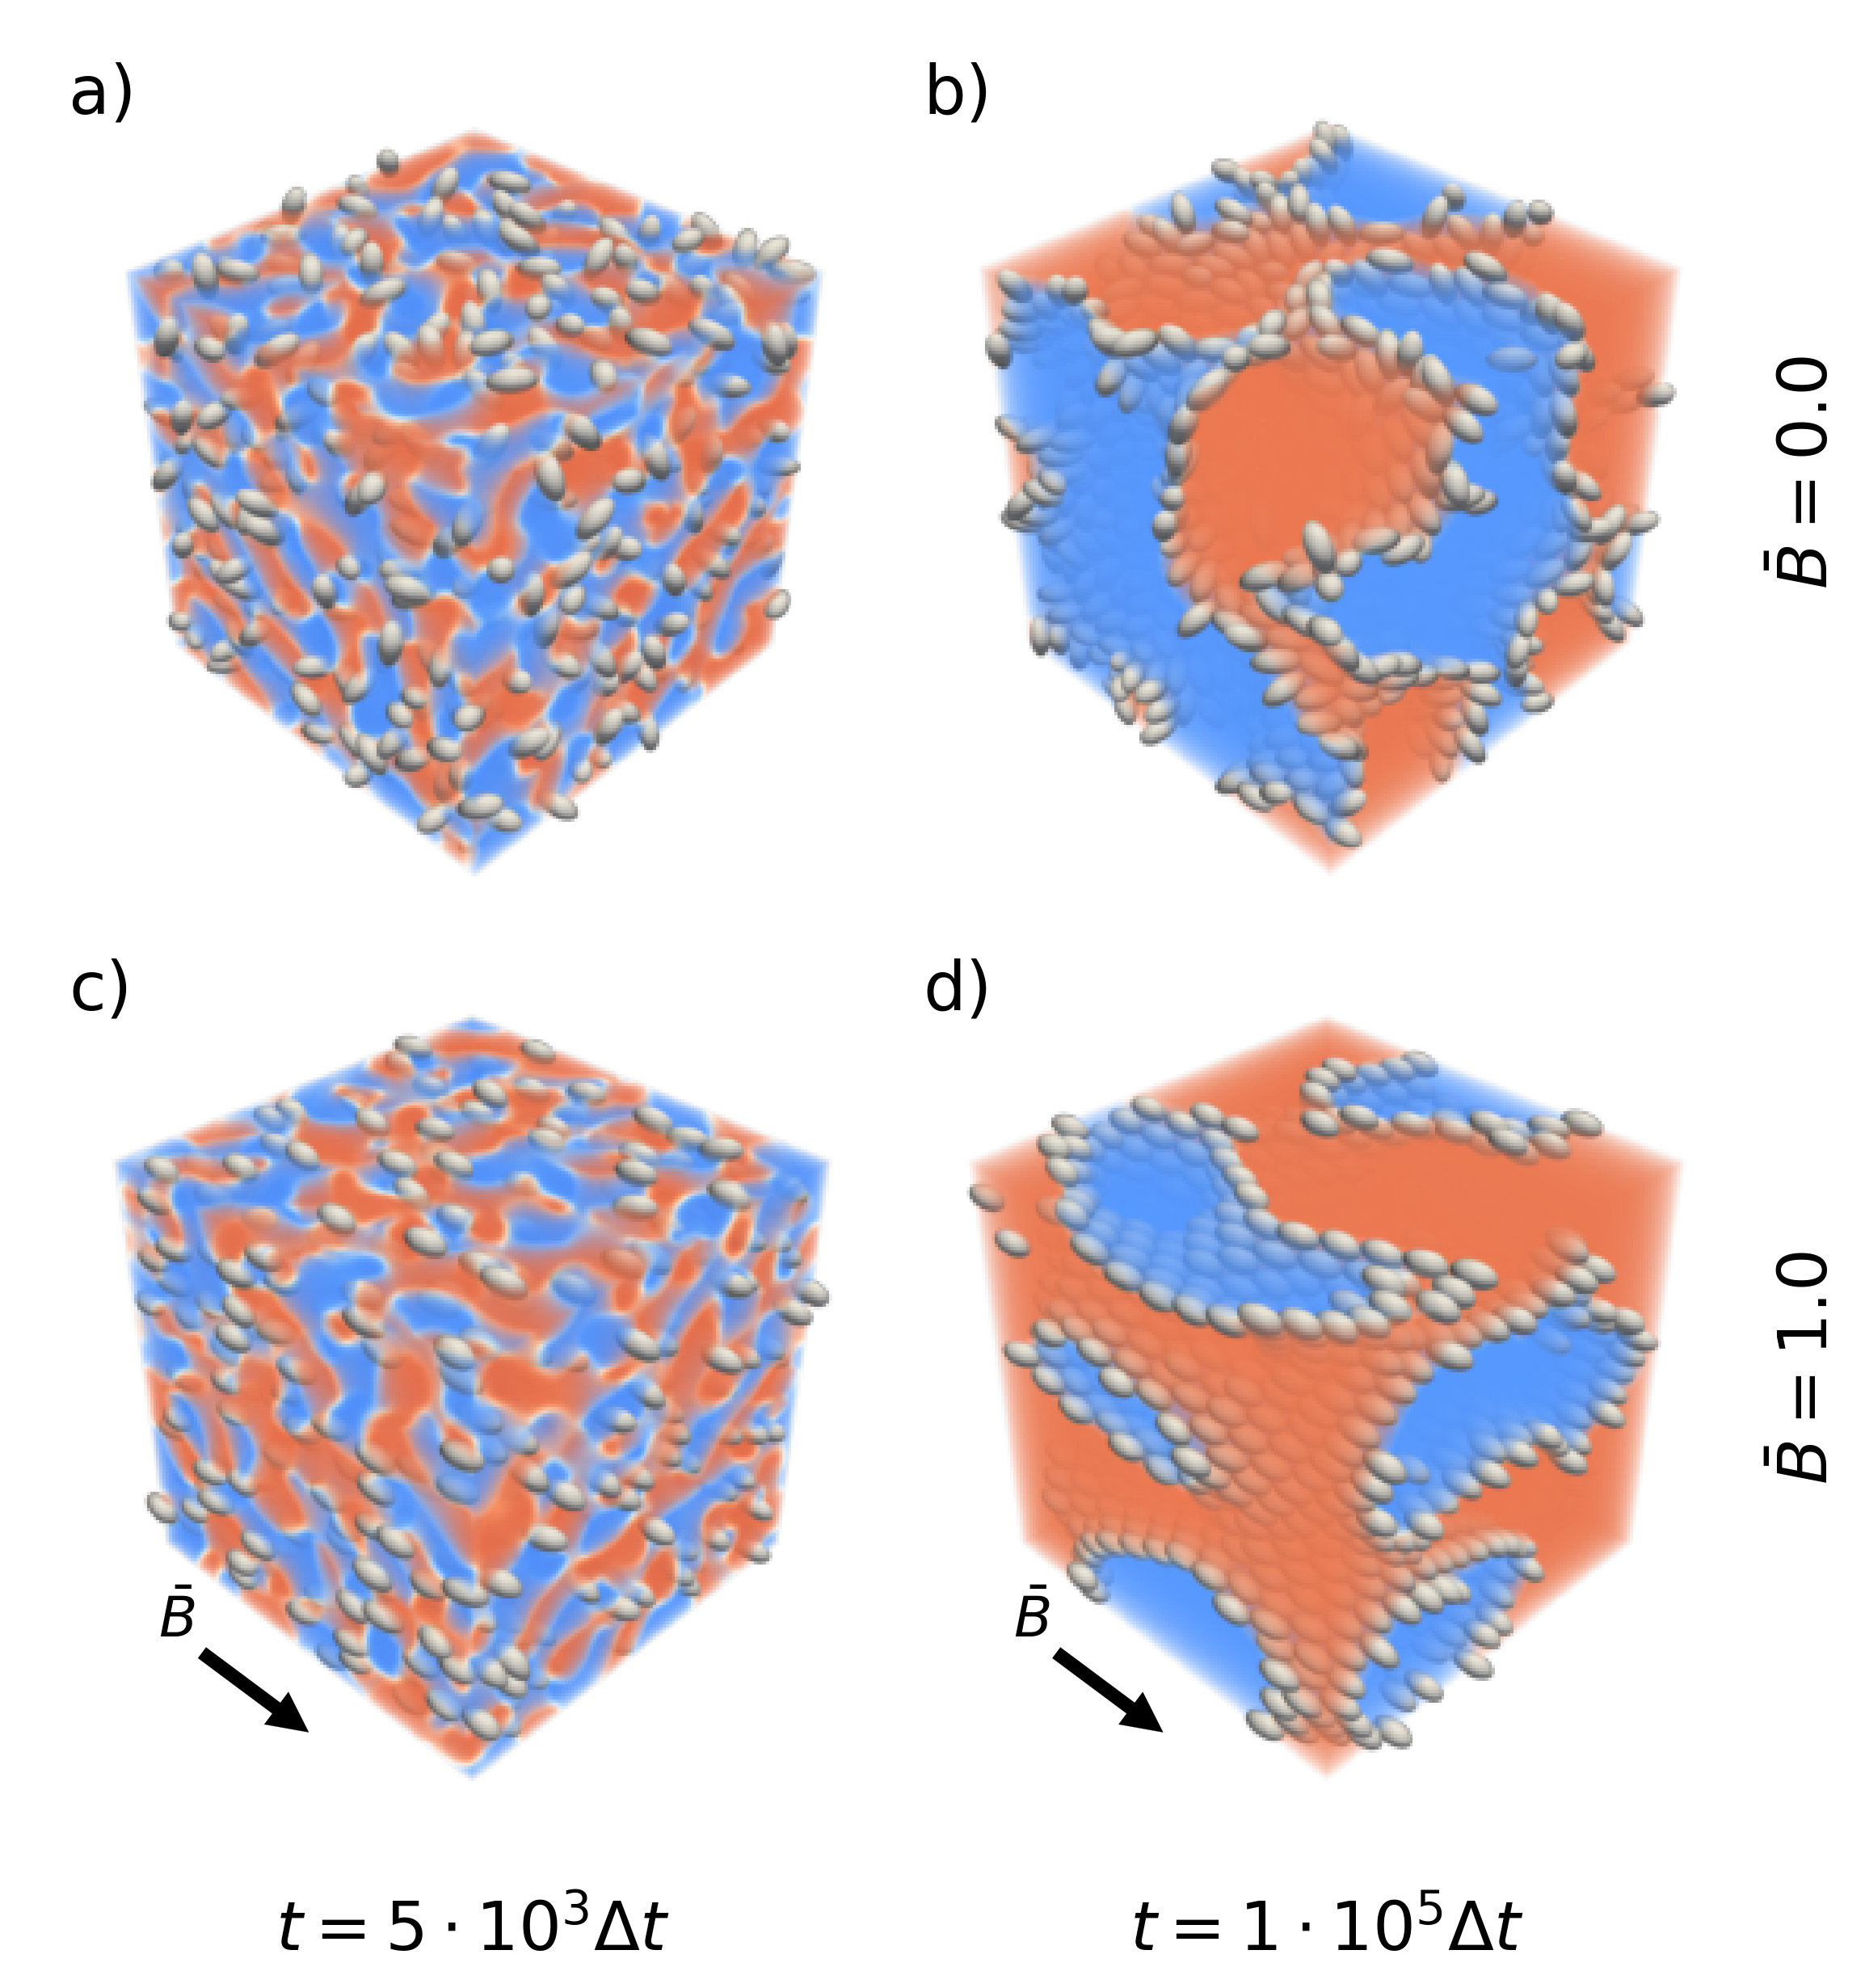
\includegraphics[width=0.5\columnwidth]{figures/results/paper1/microstructure_viz.png}
    \caption{Snapshots of emulsion gels stabilized by prolate ellipsoids after $t=5\cdot10^3$ timesteps (left) and after $10^5$ timesteps (right). The top 
             row shows the structure forming without a magnetic field. The bottom row shows the structure forming in an applied magnetic field of reduced 
             strength $\bar{B}=1.0$. The snapshots are colored according to the order parameter $\phi$.}
    \label{fig:microstructure_viz}
\end{figure}

Figure \ref{fig:microstructure_viz} presents snapshots of the bijel microstructure during formation and at the final timestep with and without magnetic fields.
The figure highlights the alignment of anisotropic particles along the field direction following its application. Particle reorientation leads to apparently larger
domain sizes in the bijels, characterized through magnetic field driven rearrangement of particles at the interface. Past work has identified how droplet coalescence
can be induced through application of magnetic fields. \cite{melle_pickering_2005} This behavior can be quantified using the domain size, done in the following section.

\begin{figure}
    \centering
    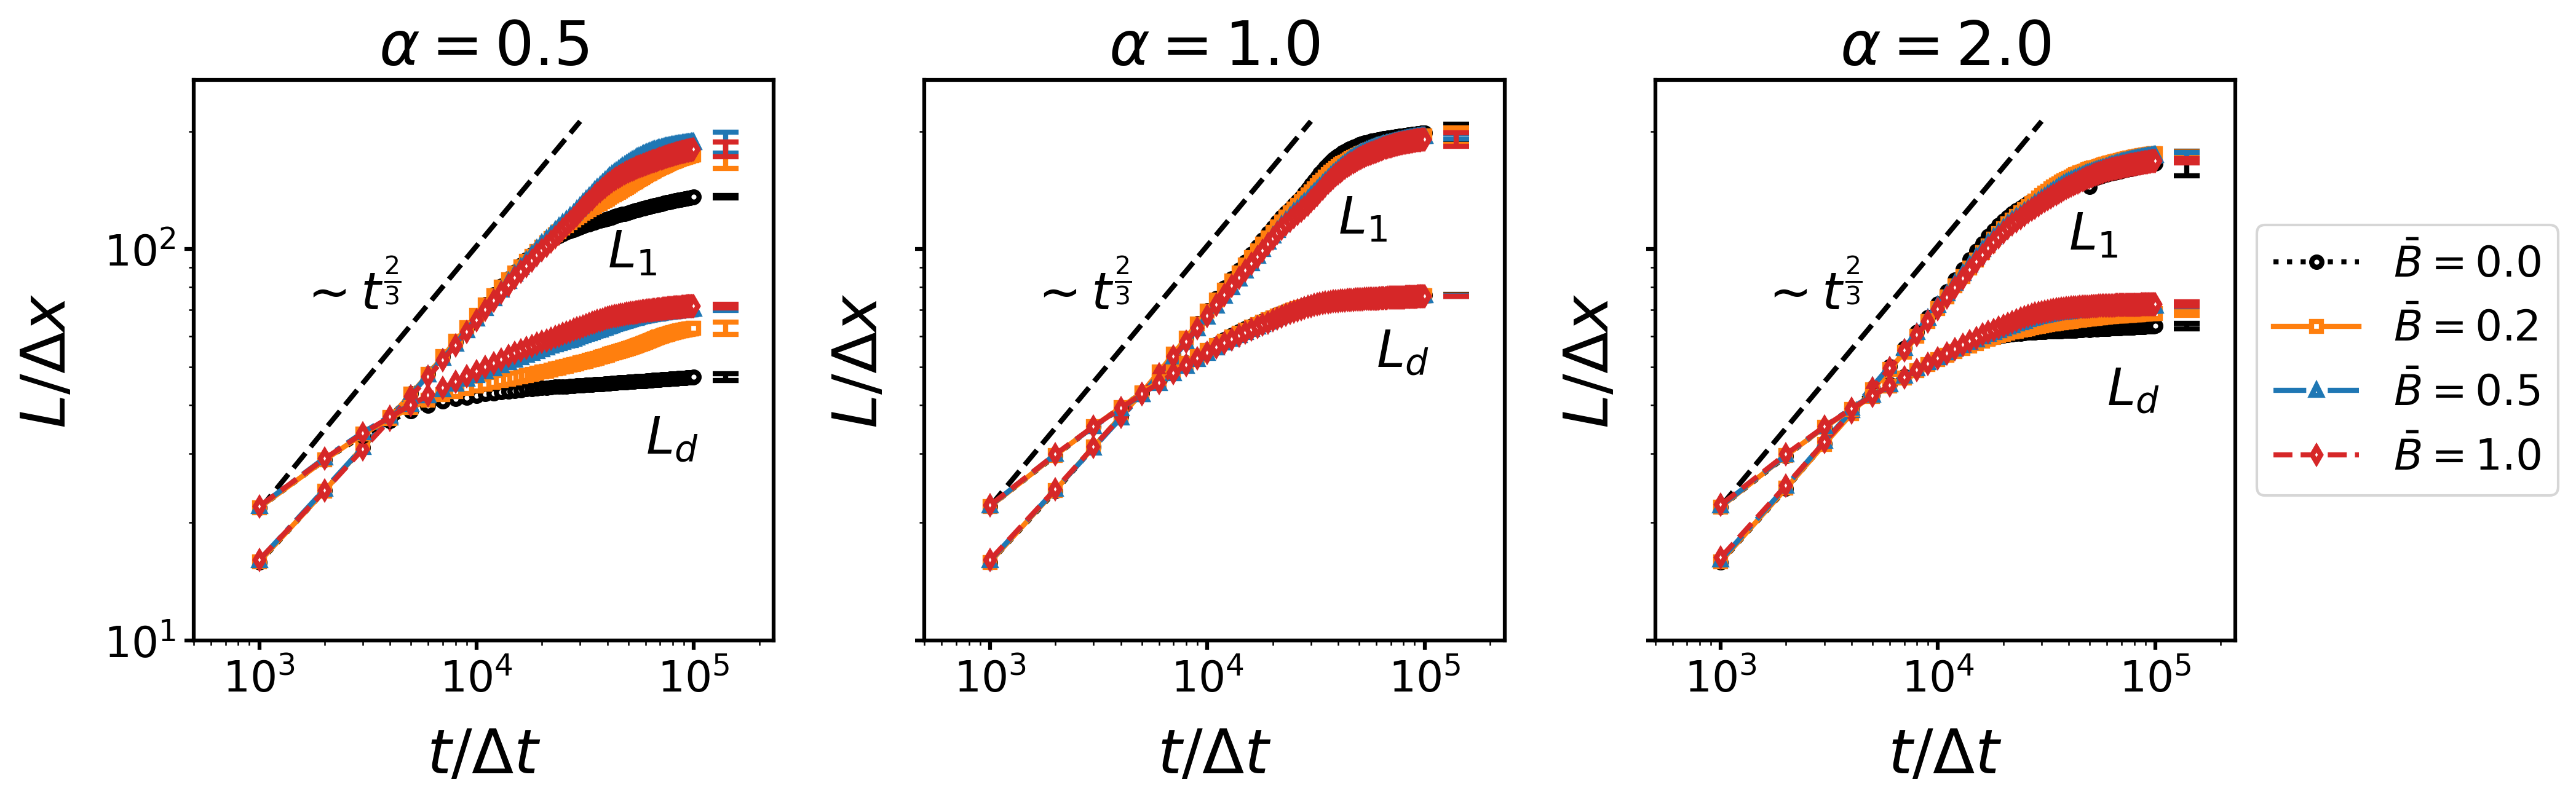
\includegraphics[width=\textwidth]{figures/results/paper1/domain_size.png}
    \caption{Time dependence of the average domain size of the bijel for different particles shapes $\alpha$ and at different magnetic 
             field strength $\bar{B}$. $L_1$ denotes the domain size obtained from the first moment of the spherical average structure 
             factor, and $L_d$ denotes the domain size obtained from the second moment of the 3D structure factor. The increase roughly 
             follows a $\sim t^{2/3}$ scaling law indicative of the inertial regime of spinodal decomposition. Image courtesy of Ulf D. Schiller}
    \label{fig:domain_size}
\end{figure}

Two methods have been identified to characterize the domain size of bijels from the structure factor. They are the first moment of the spherically averaged structure factor
named $L_1$ and the second moment of the directional structure factor. The numerical average of the second moment derived structure factor is named $L_d$. Comparing the time
evolution of both in Figure \ref{fig:domain_size}, the domain size increases before slowing down and finally plateauing. This indicates unhindered spinodal decomposition at
early times, followed by a slowdown of domain coarsening caused by particle interactions before the bijel microstructure jams. Comparing the characterized domain sizes, 
$L_d \~ 80$ compared to $L_1 \~ 150$. $L_d$ and $L_1$ also have differing time evolution, with $L_d$ beginning to plateau earlier than $L_1$. To identify which lengthscale 
should be used to characterize the time evolution of the structure, we invoke dynamical scaling.

From dynamical scaling, spinodal decomposition of binary fluids can be characterized through the inertial regime $L \~ t^{2/3}$, crossover regime $L \~ t^{n}, 2/3 < n < 1$ and 
the inertial regime $L \~ t$. \cite{kendon_3d_1999,kendon_inertial_2001} These scaling regimes can be obtained from the Navier Stokes equation with additional surface tension 
forces. The characterized lengthscales should conform to dynamical scaling as it is independent of the method used to characterize the lengthscale. By fitting the first phase
of the domain size evolution for all particle shapes, the scaling exponent of domain size change characterized with $L_1$ is found to be approximately $L \~ t^{2/3}$. However
the scaling exponent for $L_d$ is found to be $L \~ t^{0.2}$. Therefore, $L_1$ is selected to characterize the time evolution of the domain size. However the second moment of
the domain size allows characterization of the domain size in each cartesian direction. The second moment derived domain size will be used to characterize the microstructure
of the bijel.

\subsection{Effect of magnetic field on bijel microstructure}

From figure \ref{fig:domain_size}, the jamming of the bijels were determined to occur after $\~50000$ timesteps, characterized as a plateauing
of the domain size. Qualitative differences in the domain size were observed in Figure \ref{fig:microstructure_viz} which originate from particles
reorienting to the direction of the applied field. To characterize the microstructure at the final timestep, we plot the domain size of the bijels
stabilized by ellipsoidal particles and compare them to what is obtained with spherical particles. We also compare the results obtained from the
first and second moment derived structure factors by plotting the directional domain sizes as a function of the applied field to characterize
domain anisotropy. An additional simplification is made where the domain size parallel to the magnetic field is defined as $L_{\parallel}=L_z$
and the average of the other domain sizes are defined as $L_{\perp} = \frac{L_x+L_y}{2}$. 

\begin{figure}
    \centering
    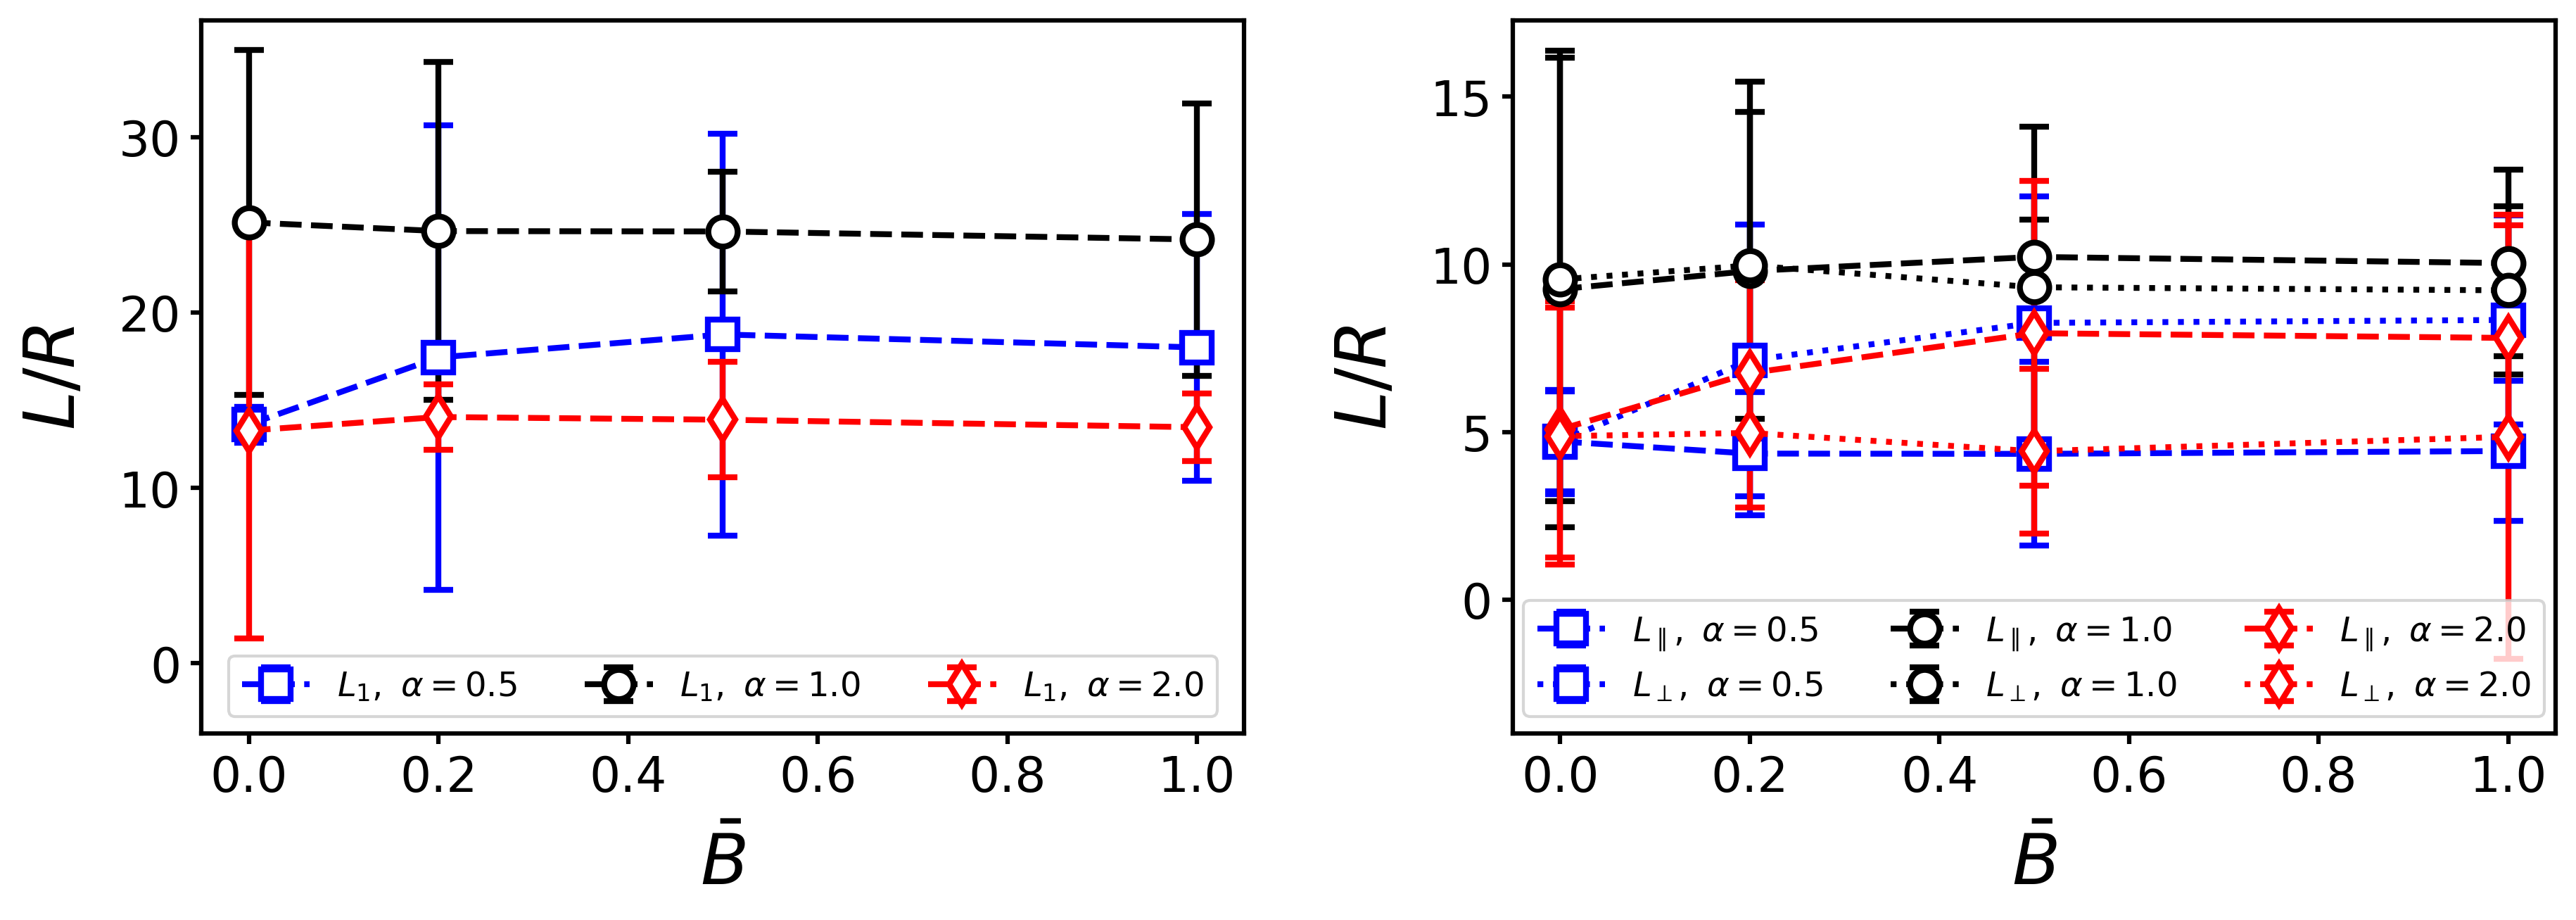
\includegraphics[scale = 0.4]{figures/results/paper1/D2a-vs-B_ss.png}
    \caption{Dependence of the average domain size on the magnetic field strength $\bar{B}$. The left plot shows the average domain size $L_1$ obtained from the spherically averaged structure factor. 
    The right plot shows the parallel and perpendicular domain size obtained from the respective second moments of the 3D structure factor. Errorbars indicate the standard deviation taken over 
    three independent simulation runs. For anisotropic particles, the directional domain size becomes more anisotropic with increasing field strength.}
    \label{fig:D2a_B}
\end{figure}

Figure \ref{fig:D2a_B} demonstrates that the first moment derived structure factor shows little change in the domain size as a function of the applied field for
all particle aspect ratios. The second moment derived domain sizes demonstrate that the application of magnetic fields create domain anisotropy in the microstructure
of bijels stabilized by ellipsoidal particles. Domain anisotropy is characterized as a divergence in the parallel and perpendicular domain sizes, seen in bijels
stabilized by ellipsoidal particles but not in bijels stabilized by spherical particles upon application of a magnetic field. The characteristics of this divergence
also differ for bijels stabilized by prolate particles and oblate particles. Bijels stabilized by prolate particles see an increase in $L_{\parallel}$ and a decrease in
$L_{\perp}$ upon application of a magnetic field, while bijels stabilized by prolate particles see the opposite. This response is also dependent on the applied field,
with the degree of response increasing from $\bar{B} = 0$ to $\bar{B} = 0.5$ before plateauing with field strengths applied above $\bar{B} = 0.5$.
The particle aspect ratio dependent response arises from the differences in the orientation of
the magnetic moment in prolate and oblate ellipsoids. In our simulations, the symmetry axis of prolate and oblate particles lies parallel to the long axis 
and short axis of the particle respectively. In addition to the geometrical constraints imparted by the shape of the particles, this results in the orientation of the
particles to differ upon application of the magnetic field.

\subsection{Tortuosity}

In Figure \ref{fig:D2a_B}, we quantitifed how the application of constant magnetic fields affects the microstructure of bijels stabilized by ellipsoidal particles
and demonstrated that microstrucutre anisotropy is generated as a function of the applied field and the particle aspect ratio. Another parameter that controls the
performance of porous materials is the tortuosity, characterized as the ratio between the parameter of interest in that system and the parameter of interest in
the bulk system. While multiple definitions exist such as the geometric, hydraulic and diffusive tortuosity exist, we use the diffusive tortuosity due to its
importance in characterizing porous material performance. A lower diffusive tortuosity in battery materials have been found to improve ion transport, reducing the
likelihood of Lithium dendrite formation and improving the charging speed and number of cycles before battery degradation. 
\cite{chen_tortuosity_2020, ebner_tortuosity_2014}. We calculate the using the method described in Section \ref{section:tortuosity}


\begin{figure}
    \centering
    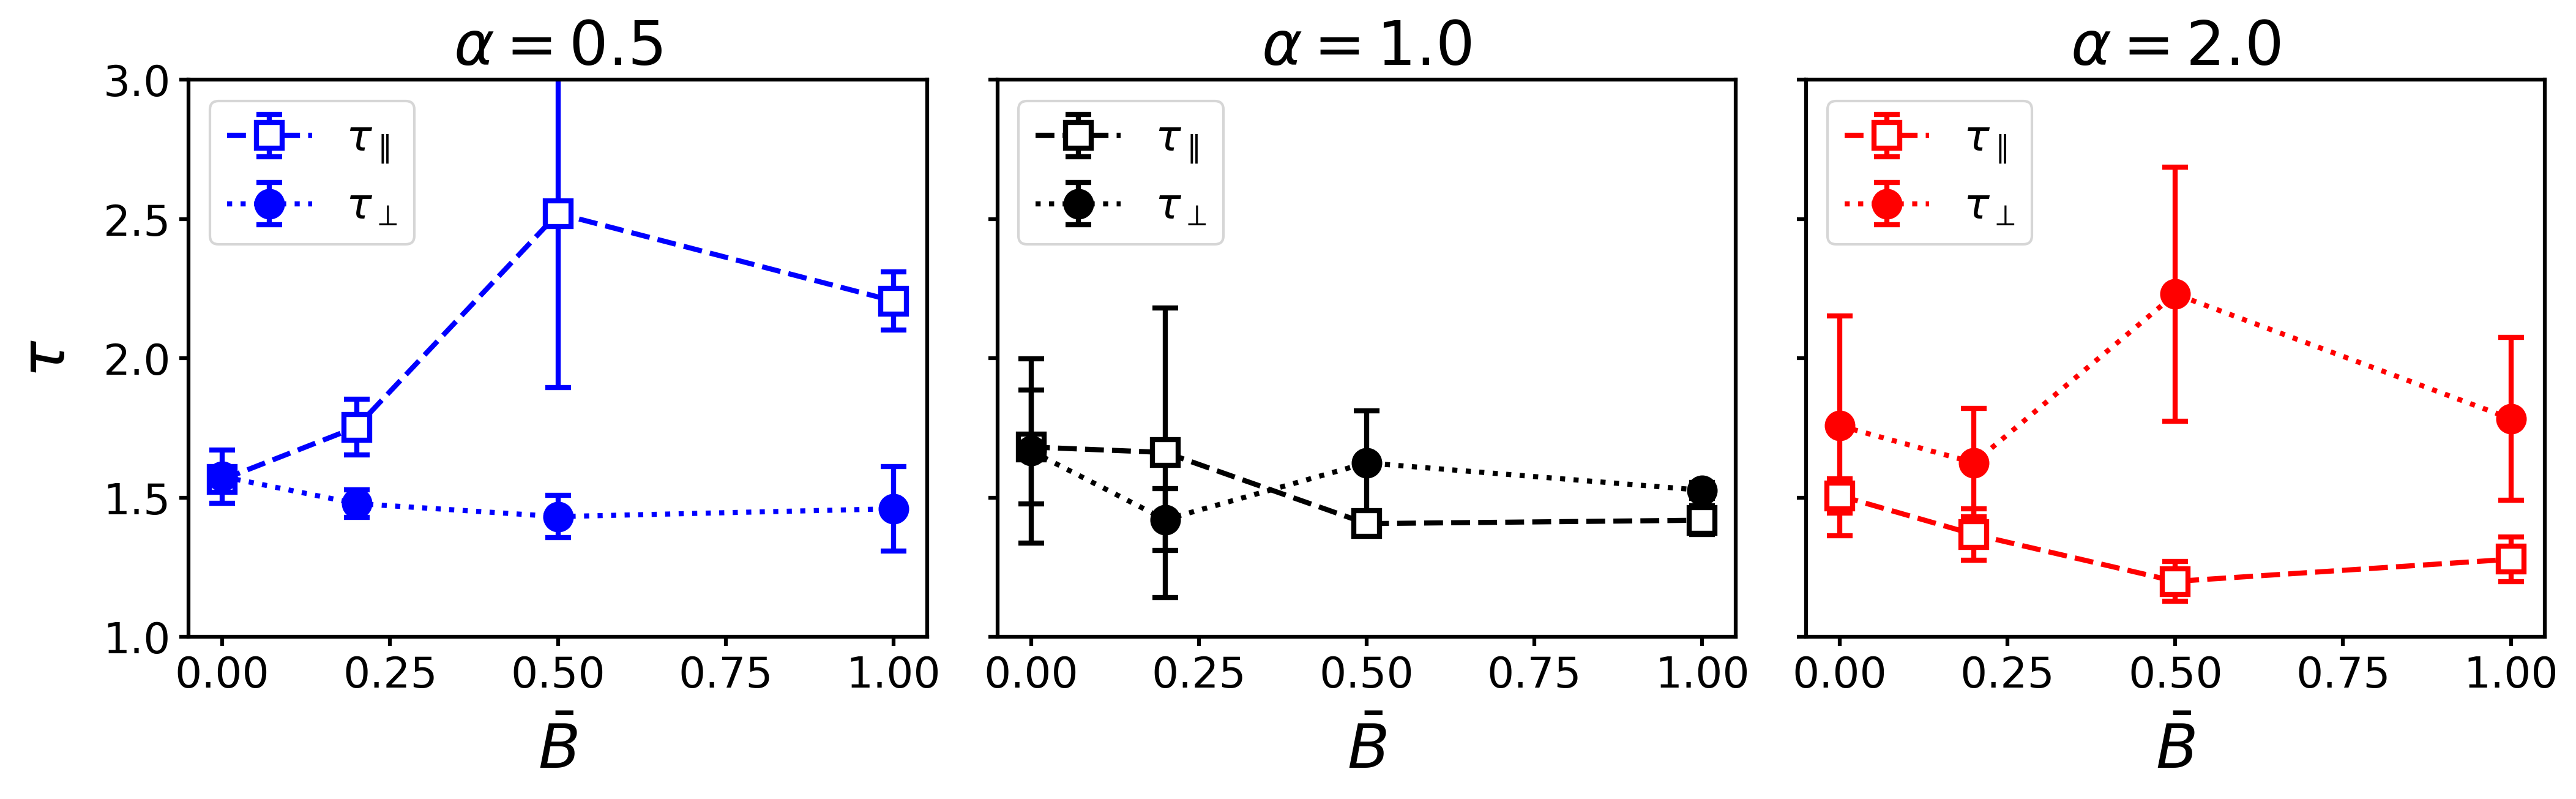
\includegraphics[scale = 0.4]{figures/results/paper1/tortuosity_compare.png}
    \caption{Dependence of the tortuosity on the magnetic field strength $\bar{B}$ for different particle shapes $\alpha$. 
             Different components of the tortuosity tensor show the anisotropy for oblate and prolate particles.}
    \label{fig:tau_B}
\end{figure}

From Figure \ref{fig:tau_B}, the tortuosities calculated for bijels stabilized by spherical particles 

\subsection{Curvature}

Beyond the length scale, curvature analysis offers insights into the
topological landscape of the bijel, facilitating further
microstructure optimization for various applications.
\cite{reeves_quantitative_2016} We plot the area averaged mean and
gaussian curvature \(H\Sigma^{-1}\) and \(K\Sigma^{-2}\) for bijels
stabilized with oblate, spherical and prolate ellipsoids at the final timestep in Figure
\ref{fig:curvature-vs-B_ss}. 

\begin{figure} 
    \centering 
    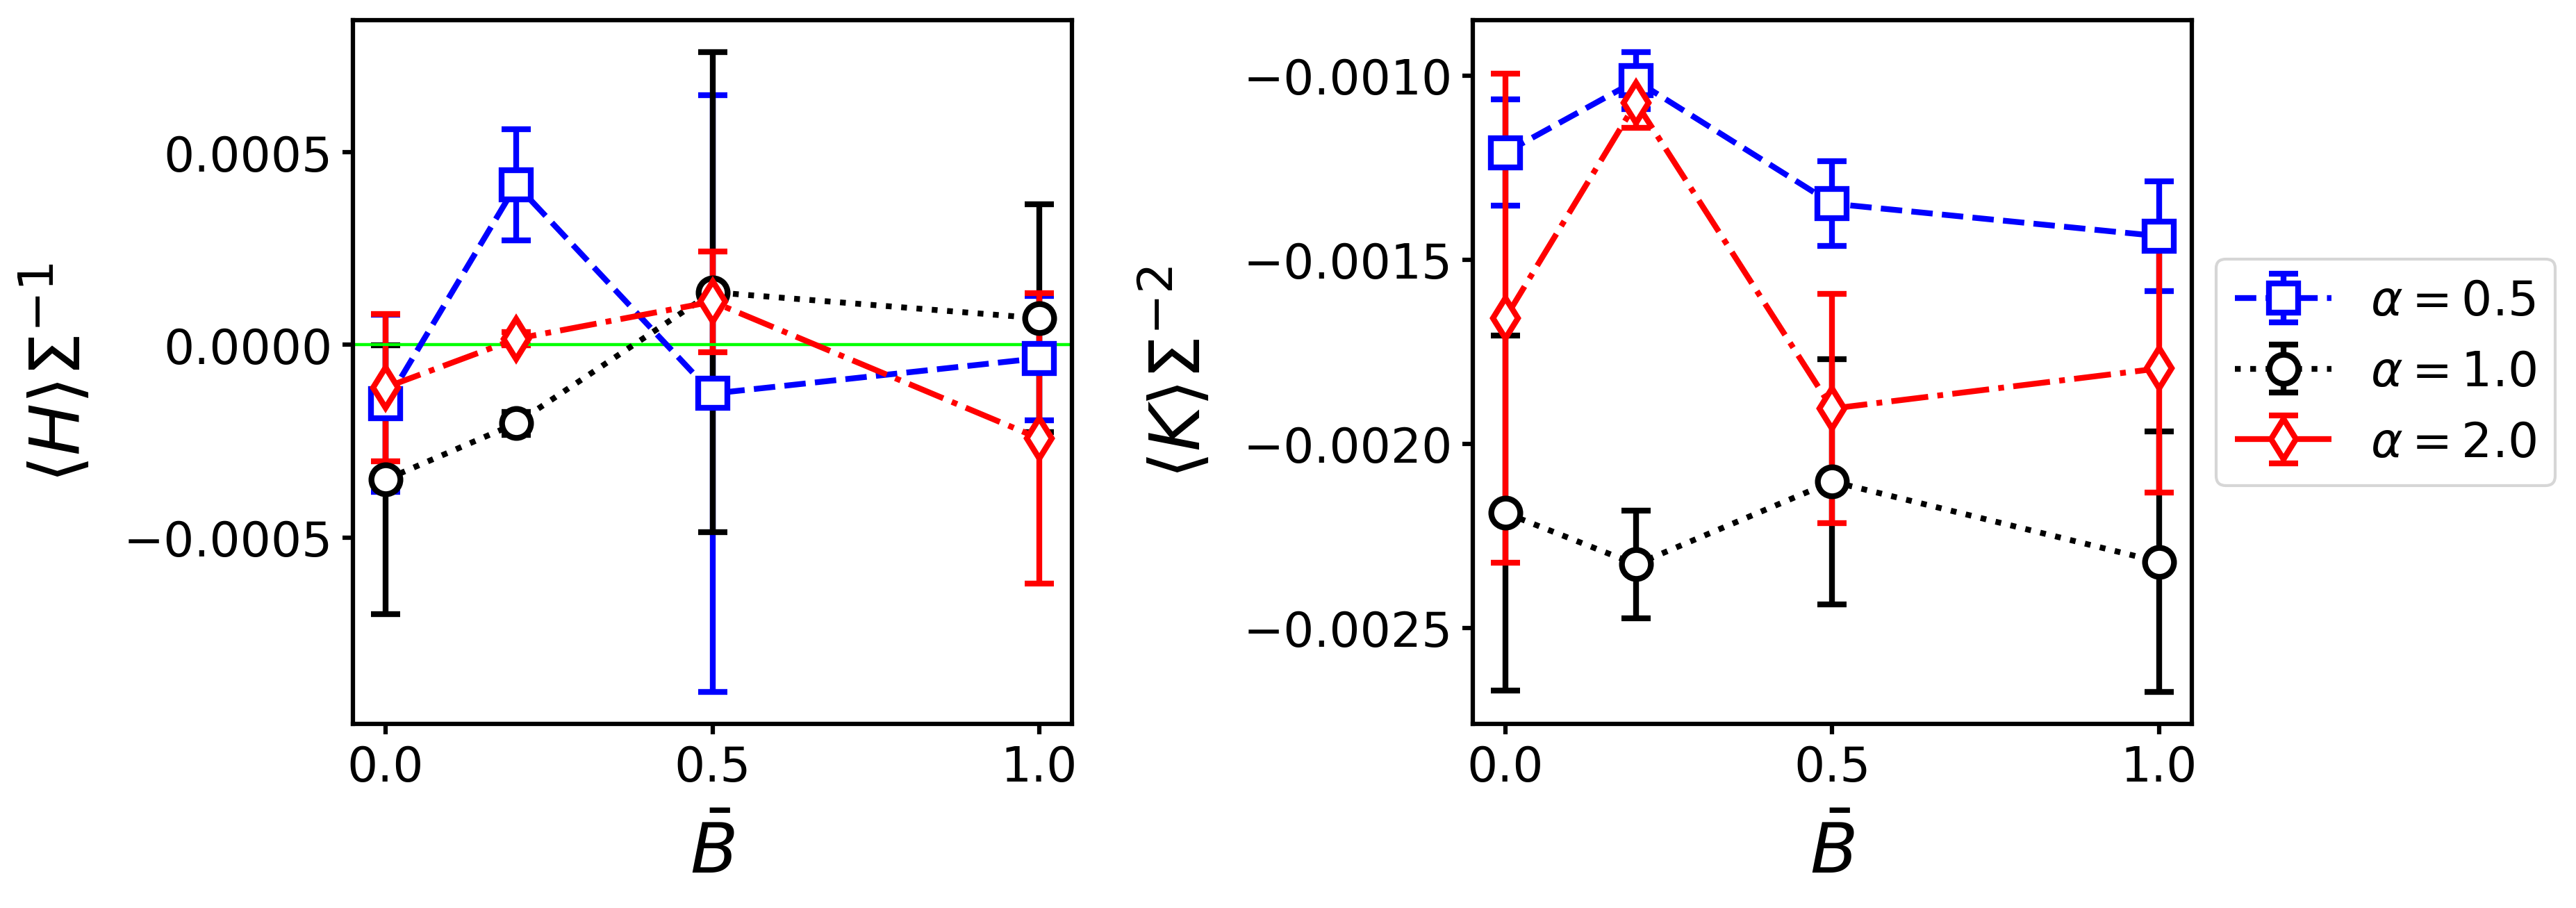
\includegraphics[scale = 0.4]{figures/results/paper1/curvature-vs-B_ss.png} 
    \caption{Plot of the area averaged mean $\langle H \rangle \Sigma^{-1}$ and Gaussian 
            $\langle K \rangle \Sigma^{-2}$ curvature in the left and right respectively. Each 
            plot contains the $\langle H \rangle \Sigma^{-1}$ and $\langle K \rangle \Sigma^{-1}$ 
            at the final timestep averaged across 3 runs for particles with $\alpha = 0.5, 1, 2$. 
            The mean curvature remains 0 on average, while the Gaussian 
            curvature shows a reduction as the magnetic field strength is increased for 
            ellipsoidal particles.} 
    \label{fig:curvature-vs-B_ss}
\end{figure}

Error bars are represented by the standard
deviation of the three simulations per parameter set performed. The area
averaged mean curvature shows little dependence on the applied field
strength with values around 0 and within error of one another. A value
near or at 0 is expected as the fluid volume fraction is equal and the
particles are neutrally wetting, implying the interface should not have
a preferred direction of curvature. \cite{jinnai_interfacial_2001} For
ellipsoidal particles, the gaussian curvature becomes more negative as
larger field strengths are applied. We also see that the gaussian
curvature becomes more positive as the interfacial area of the particle
increases. The trend of these results are inverse to the interfacial
area of each particle, \(A_{rm}\). This is expected behavior and is in
agreement with experiments that have investigated the effect of particle
size on the curvature of bijels. \cite{reeves_quantitative_2016}

To explain the reduction in $\langle K\Sigma^{-2} \rangle$ as a function of the applied field strength, two mechanisms are proposed. The first is that 
the particle alignment to the magnetic field during coarsening changes the topology of the surface, which upon jamming of ellipsoidal particles is locked in. 
The other proposed mechanism is that the time evolution of spinodal decomposition remains unaffected, but that the interface conforms to the magnetic field 
driven arrangement of particles upon jamming. While we cannot apply the Gauss Bonnet theorem to characterize the results, we can still relate the coarsening 
behavior of the bijel through its change in genus to the curvature. The time evolution of the genus serves as a topological technique to characterize the 
coarsening of the bijel, which alongside the $\langle K\Sigma^{-2} \rangle$, allows us to identify deviations from the coarsening behavior of bijels 
stabilized with spherical particles, and with magnetic fields. We calculate the genus by extracting the isosurface of the filled order parameter, where 
$\phi = 0$. It is then meshed using the marching cubes algorithm implemented in scikit-image with a cube size of 1. \cite{van2014scikit} From the vertices(v) 
and faces(f) generated from the marching cubes algorithm, we calculate the number of edges(e). The Euler Poincare characteristic, $\chi = n + f - e$. The genus is 
then obtained from the Euler Poincare parameter as $g = 1 - \chi/2$.

\begin{figure} 
    \centering 
    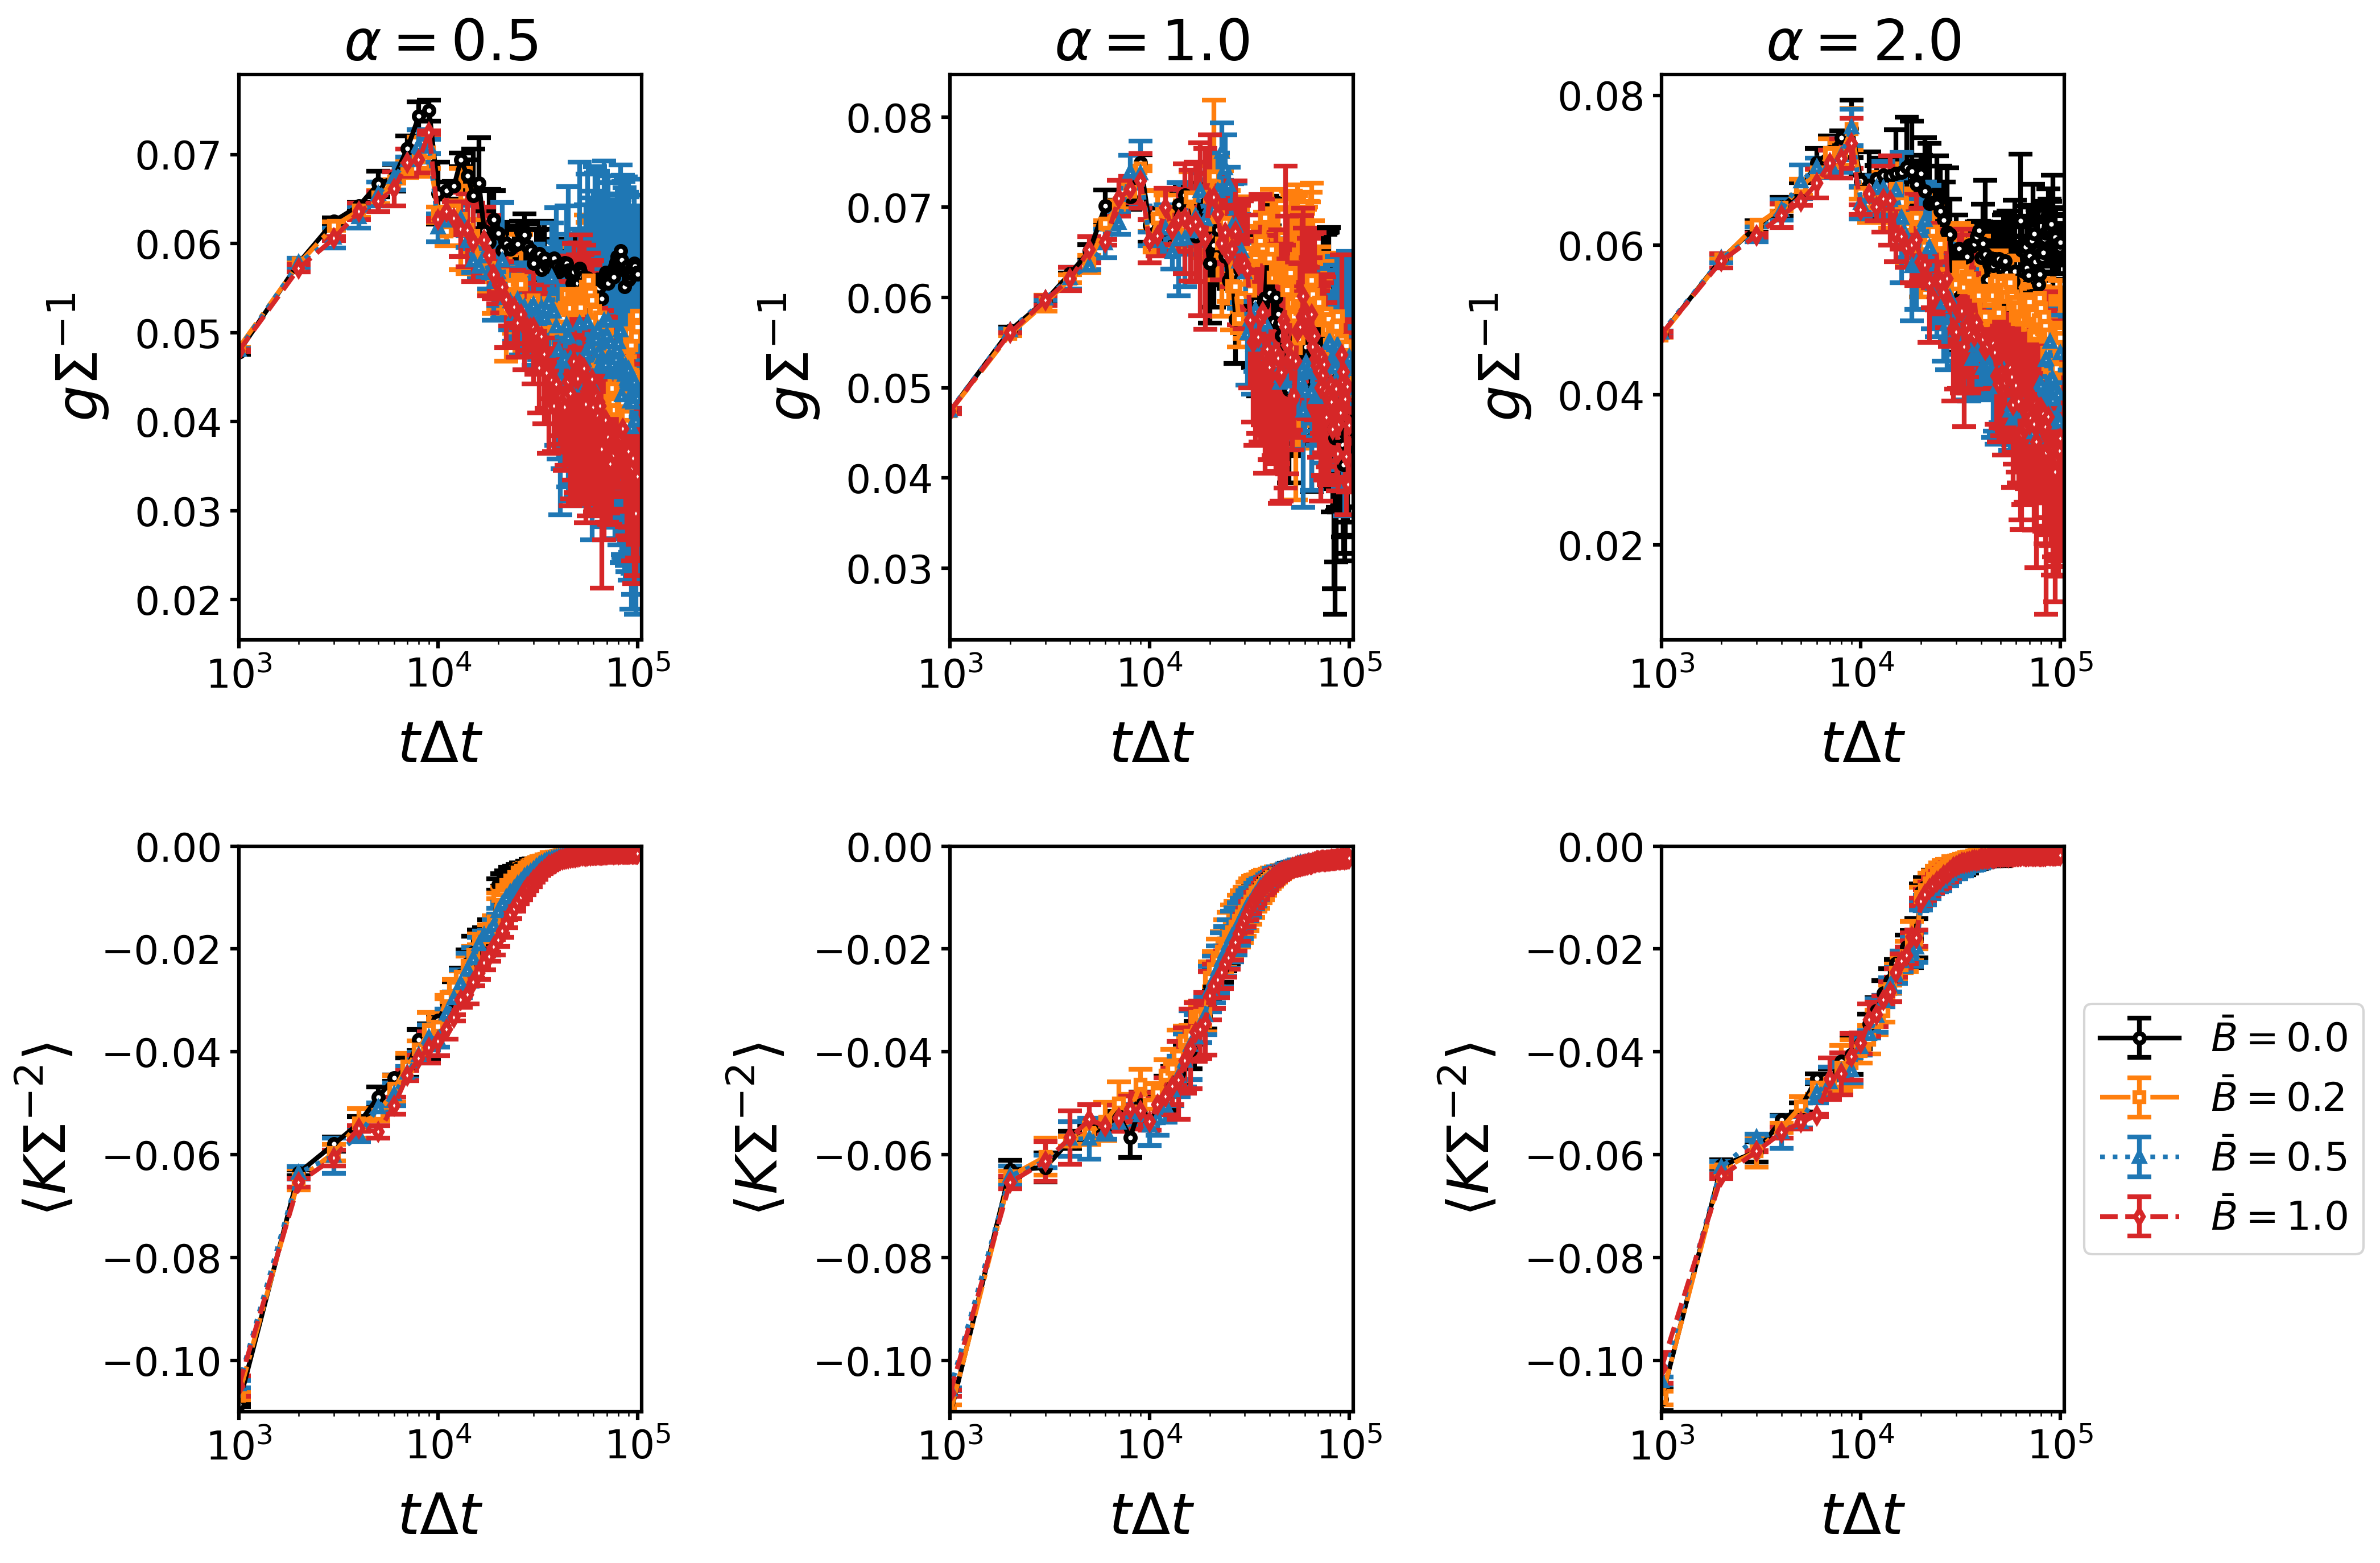
\includegraphics[scale = 0.4]{figures/results/paper1/genus_curvature_vs_coverage.png} 
    \caption{Plots of Gaussian $\langle K \rangle \Sigma^{-2}$ curvature over time averaged across 3 runs. 
    From left to right, We have particles with $\alpha = 0.5, 1, 2$. We observe that the initial stages of 
    evolution are unaffected by the applied magnetic field. However, after about 10000 timsteps, We see a 
    magnetic field dependence on the evolution of the Gaussian curvature. The preservation of this divergence 
    occurs when ellipsoidal particles are used but not spherical particles.} 
    \label{fig:curvature_vs_coverage}
\end{figure}

The time evolution of $g \Sigma^{-1}$ of bijels stabilized with spherical particles is unaffected by the application of a magnetic field. However, a 
slight decrease in the genus as a function of the applied field is observed for bijels stabilized with ellipsoidal particles. This suggests that the 
evolution of the surface corresponding to the interface is changed by the adsorption and orientation of magnetically responsive ellipsoidal particle. 
We see effects of this change in $\langle G \rangle \Sigma^{-2}$ where we see the evolution of the curvature being delayed, indicated as a rightward 
shift of the plots as a function of the applied field. 

Despite all our curvature calculations being normalized with their surface area to volume ratio, we still see curvature differences as a function of the applied 
magnetic field. Experiments have identified that curvature changes can occur due to the formation of monogels, which are particle networks formed from bijels that 
can withstand the remixing of their constituent liquids. \cite{sanz_colloidal_2009, lee_making_2013} This process cannot occur in our simulations as we am utilizing 
electrically neutral particles that only interact through contact forces. Therefore, the change in curvature arises from microstructure changes driven by particle 
alignment to the magnetic field direction. These results provide support for the mechanism of control being due to particle alignment to the magnetic field during 
coarsening changes the topology of the surface, which upon jamming of ellipsoidal particles is locked in. As our particles only interact through contact forces, 
the only mechanism present that can change the topology of the interface would be particle interactions upon contact with each other. Particle interactions are 
controlled through the orientation of particles and the local ordering of particles on the interface. Seeing that there are differences in the gaussian curvature of the bijel,
the domain anisotropy characterized in Figure \ref{fig:D2a_B} may be able to be characterized as changes in the topology of the surface. Chan and Thornton introduced a 
topological technique to characterize the connectivity of surface as a function of a distance from the interface to calculate the channel size distribution. 
\cite{chan_channel_2012} We can use the channel size distribution to investigate how the connectivity of the microstructure and thus the 
channel size is affected as a function of the applied magnetic field.

\begin{figure} 
        \centering 
        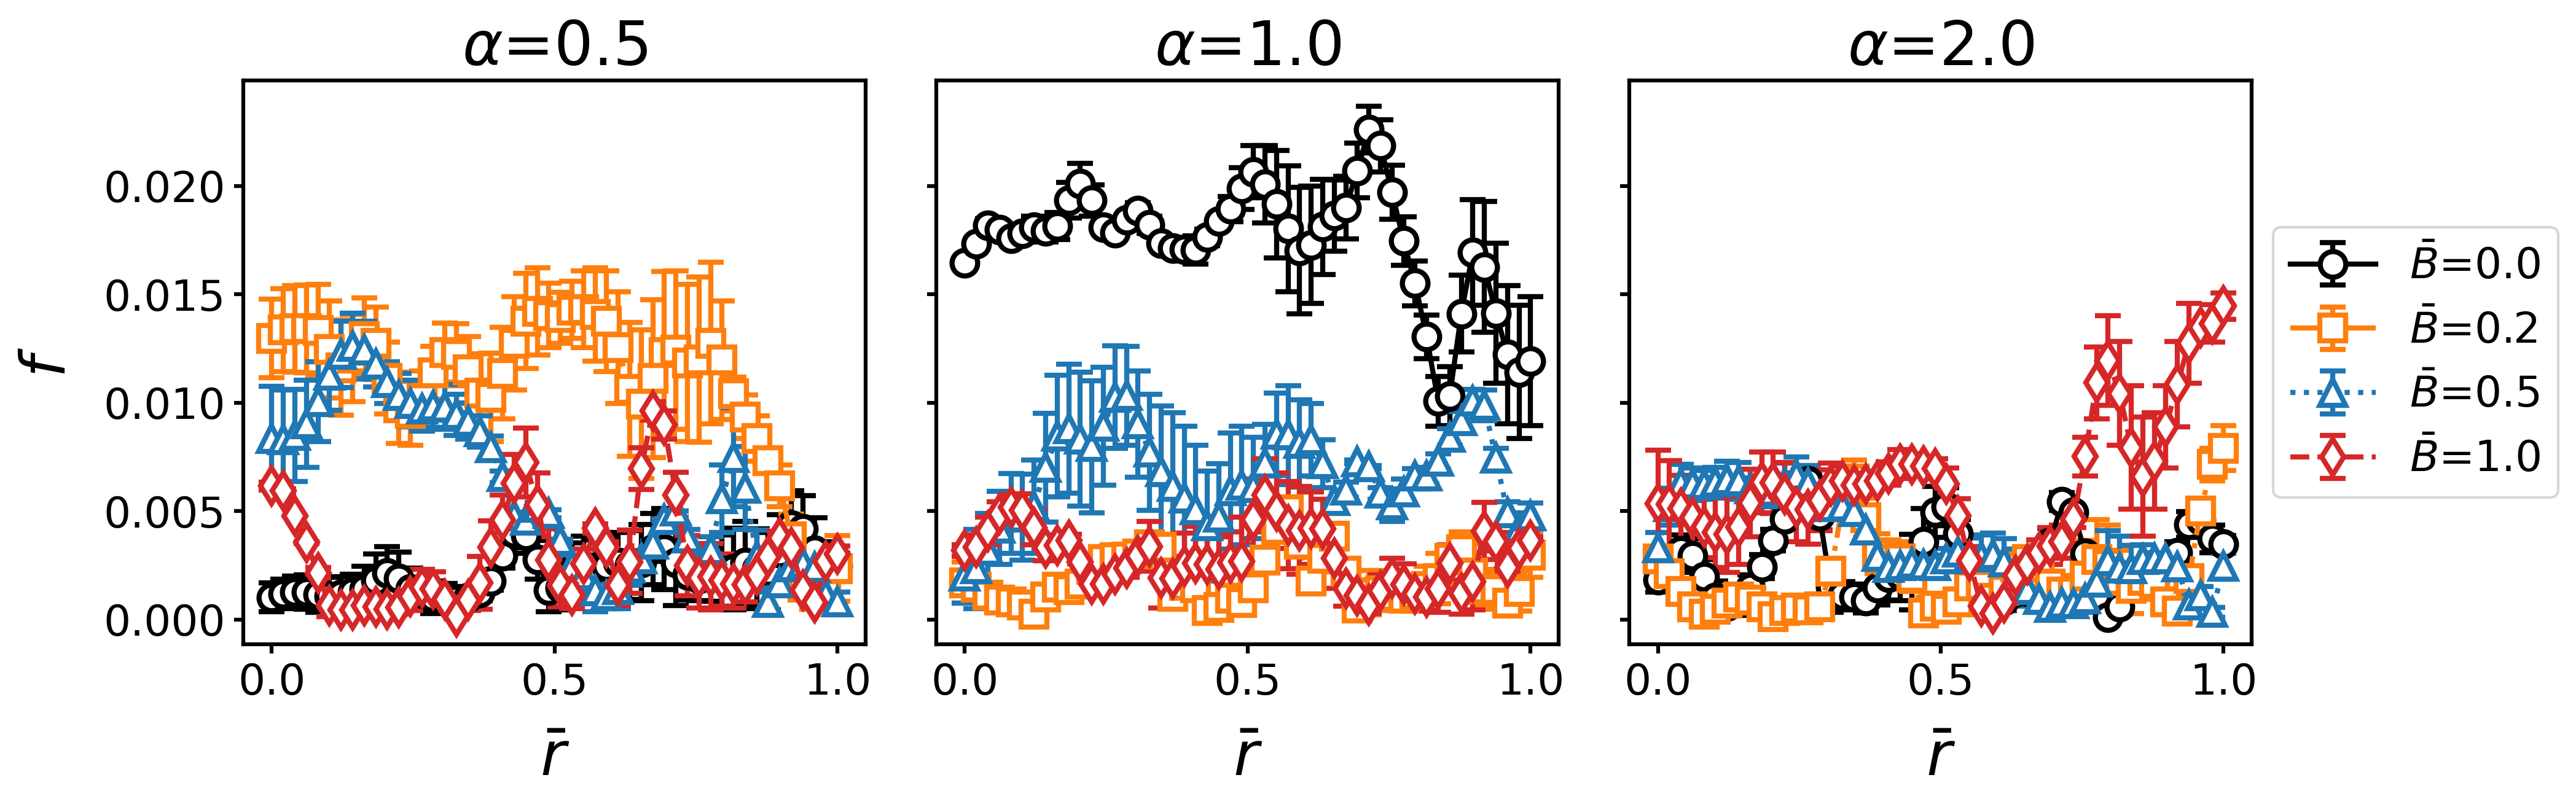
\includegraphics[scale = 0.4]{figures/results/paper1/CSD_ss.png} 
        \caption{Plots of the channel size distribution for bijels stabilized by oblate, spherical and oblate particles at the final timestep plotted
                 against the distance from the interface normalized with the characteristic length scale. The channel sizes obtained are averaged over 
                 three runs. We see that the peak locations are shifted to larger and smaller positions for bijels stabilized with ellipsoidal particles
                 upon field application} 
        \label{fig:CSD_B_ss}
    \end{figure}

While run to run variation is observed, the combined data of the channel size distribution shown in Figure \ref{fig:CSD_B_ss} shows some differences 
in the channel size distribution in each bijel stabilized with ellipsoidal particles. It was expected that the domain anisotropy obtained using second moment of the 
structure factor would manifest as two peaks in the channel size distribution. \cite{karthikeyan_formation_2024} This behavior is observed in the channel size 
distribution for bijels stabilized with ellipsoidal particles with $\bar{B} = 1$, but is more difficult to see when smaller magnetic fields are applied. 
These differences arise from the particle ordering and local distribution changes observed. 

\subsection{Kinetics of bijel formation in magnetic fields}

To shed light on the mechanisms involved in the coarsening dynamics,
we now turn to the kinetics of bijel formation in more detail. The
coarsening dynamics can be characterized by a coarsening speed. Here,
we use the finite difference of the directional domain size to
calculate the components of the coarsening velocity
%
\begin{equation}
u_{L_\beta}(t) = \frac{L_\beta(t+\Delta t_s)-L_\beta(t-\Delta t_s)}{2\Delta t_s} ,
\end{equation}
%
where \(\Delta t_s\) is the time between simulation
snapshots, and $\beta$ denotes either the direction parallel or perpendicular to the magnetic field.

\begin{figure}
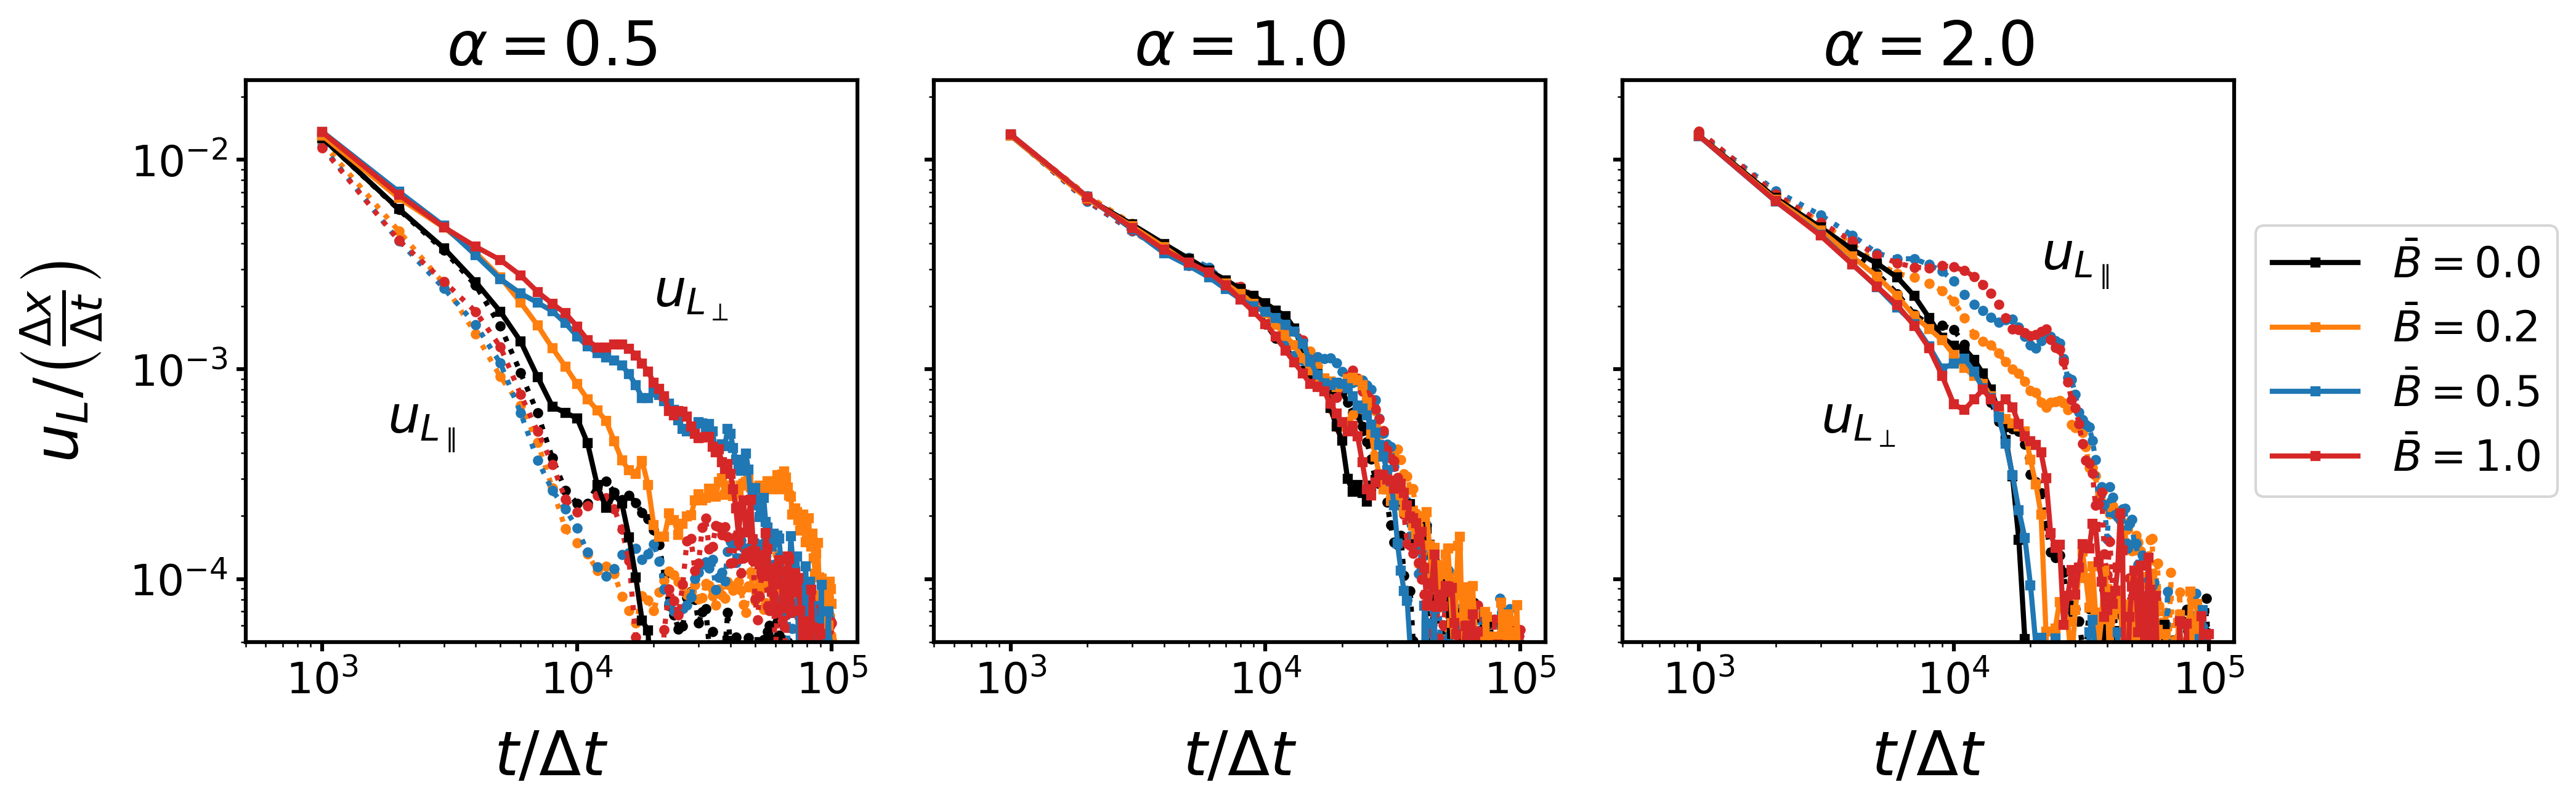
\includegraphics[width=\textwidth]{figures/results/paper1/coarsening_vel.png}
\caption{Time-dependence of the coarsening velocity $u_L$ for different particles shapes $\alpha$  
and at different magnetic field strength $\bar{B}$. The different components of the coarsening velocity 
show that the jamming time is different in the direction parallel and perpendicular to the magnetic field. Image provided
courtesy of Ulf D. Schiller.}
\label{fig:coarsening_velocity}
\end{figure}

% Figure \ref{fig:coarsening_velocity} shows the coarsening speed in the directions parallel and perpendicular to the applied magnetic field. 
% The data confirms that for spherical particles, domain coarsening remains isotropic. We observe a higher coarsening speed initially which slows 
% at later times when the particles begin to jam. This indicates that the
% coarsening is subject to different time scales, as reported previously
% by Harting and co-workers \cite{gunther_timescales_2014}. Reeves et
% al.~\cite{reeves_particle-size_2015} have pointed out that bijel
% formation hinges on the jamming time in relation to the disruption time, i.e., the time scale at which domain pinch-off events can cause bijel break-up through 
% depercolation. In our simulations, however, we have not observed disruption of bijel formation; stable bijels form for all parameters consistent with simulations 
% by Stratford et
% al.~\cite{stratford_colloidal_2005} and Jansen et al.~\cite{jansen_bijels_2011}.

% For ellipsoidal particles, our data clearly shows that an\-isotropic
% domain coarsening arises in magnetic fields.  For oblate particles
% (\(\alpha=0.5\)), the coarsening speed in the direction perpendicular
% to the field increases with increasing magnetic field strength.
% Jamming in this direction appears to be delayed compared with the
% direction parallel to the field. The coarsening speed in the parallel
% direction remains comparable to the case without an applied magnetic
% field. This anisotropic behavior of the coarsening speed reverses for
% prolate particles, where the coarsening speed in the direction parallel to the field increases with increasing field strength, and jamming in this direction
% is delayed compared with the perpendicular direction. In addition, we observe a shoulder (around \(10^4\Delta t\)) where the coarsening speed decays more slowly before jamming sets in. These results suggest that the coarsening near the jamming time is affected by a mechanism that depends on the applied magnetic field and causes the anisotropic
% behavior. This mechanisms involves the re-orientation of anisotropic
% particles and their alignment relative to the direction of the
% magnetic field. To confirm this hypothesis, we analyze the
% orientational order of the particles and their alignment relative to
% the magnetic field and the interface, respectively.

\subsection{Particle re-orientation and packing}

\begin{figure}
    \centering
    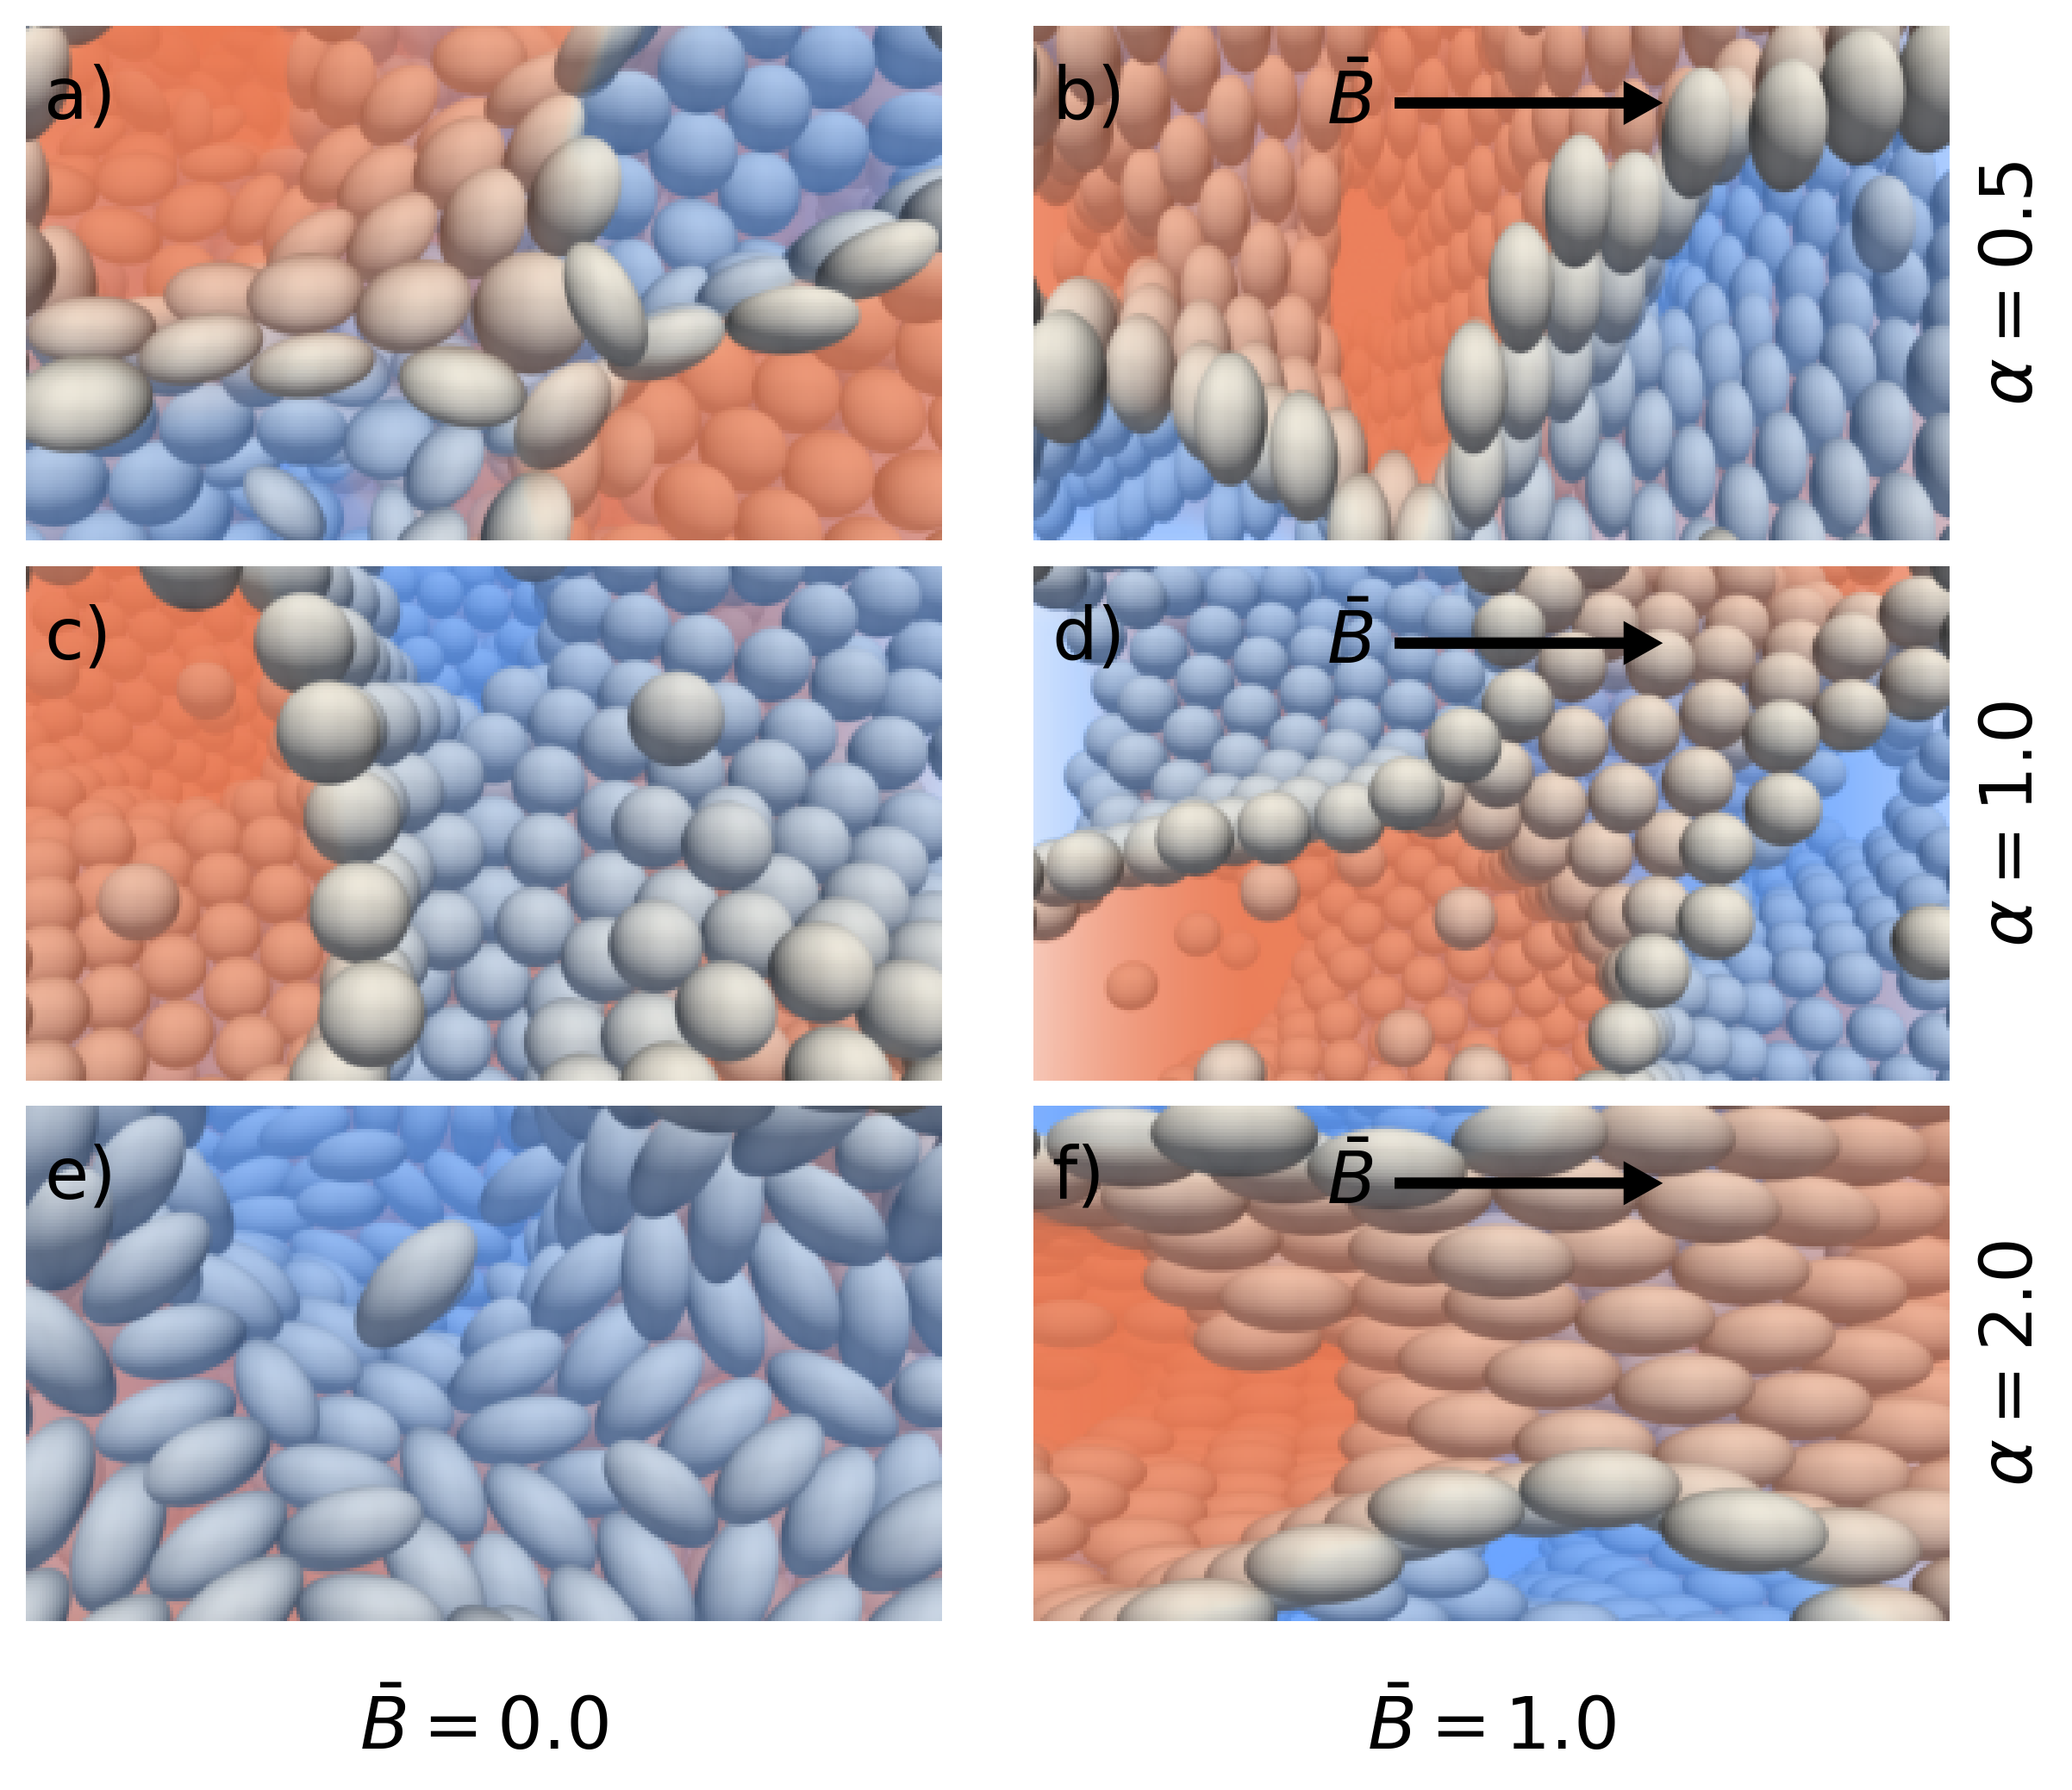
\includegraphics[width=0.5\columnwidth]{figures/results/paper1/particle_packing_viz.png}
    \caption{Snapshots illustrating the particle packing at the interface for different particle shapes $\alpha$ with (left) 
            and without (right) applied magnetic field $\bar{B}$. The right column shows the alignment of the symmetry axis of 
            the oblate (top row) and prolate (bottom row) particles in the direction of the magnetic field indicated by arrows.}
    \label{fig:packing_viz}
\end{figure}

\begin{figure}
    \centering
    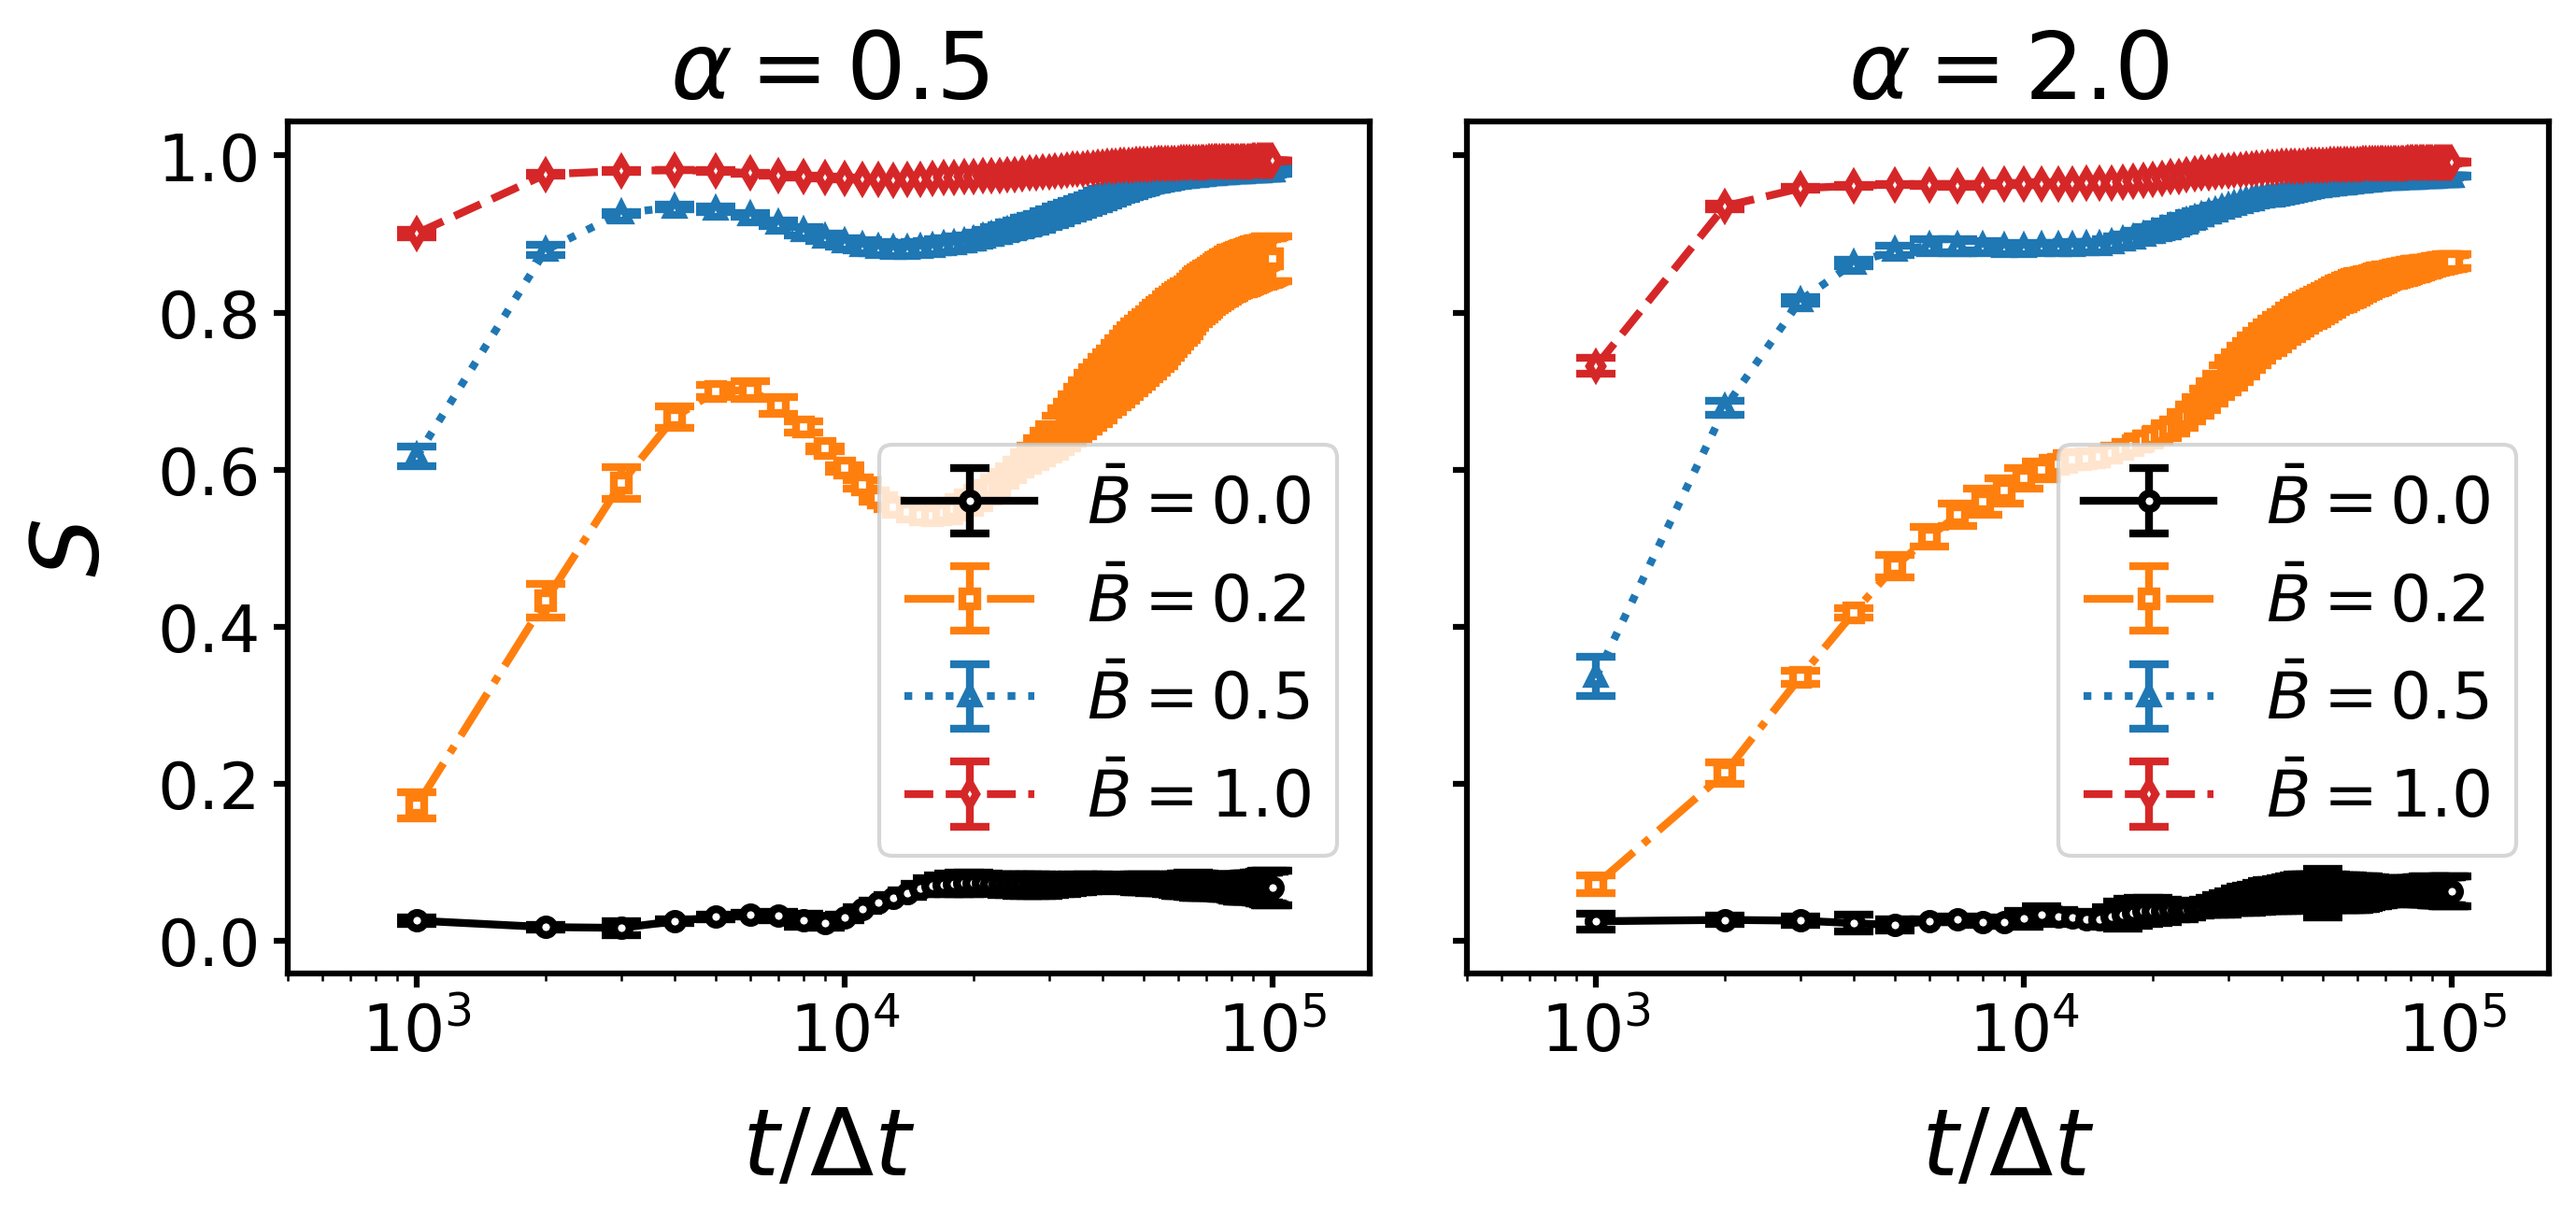
\includegraphics[scale = 0.4]{figures/results/paper1/S-vs-t.png}
    \caption{Time-dependence of the nematic order parameter $S$ of oblate ($\alpha=0.5$) and prolate ($\alpha=2$) 
            particles at different field strength $\bar{B}$. Errorbars indicate the standard deviation taken over 
            three independent simulation runs. Nematic order generally increases with applied field strength for all particle geometries. 
            The increase slows down (for prolate particles) or reverses (for oblate particles) around $10^4$ timesteps.}
    \label{fig:nematic_time}
\end{figure}


\begin{figure}
    \centering
    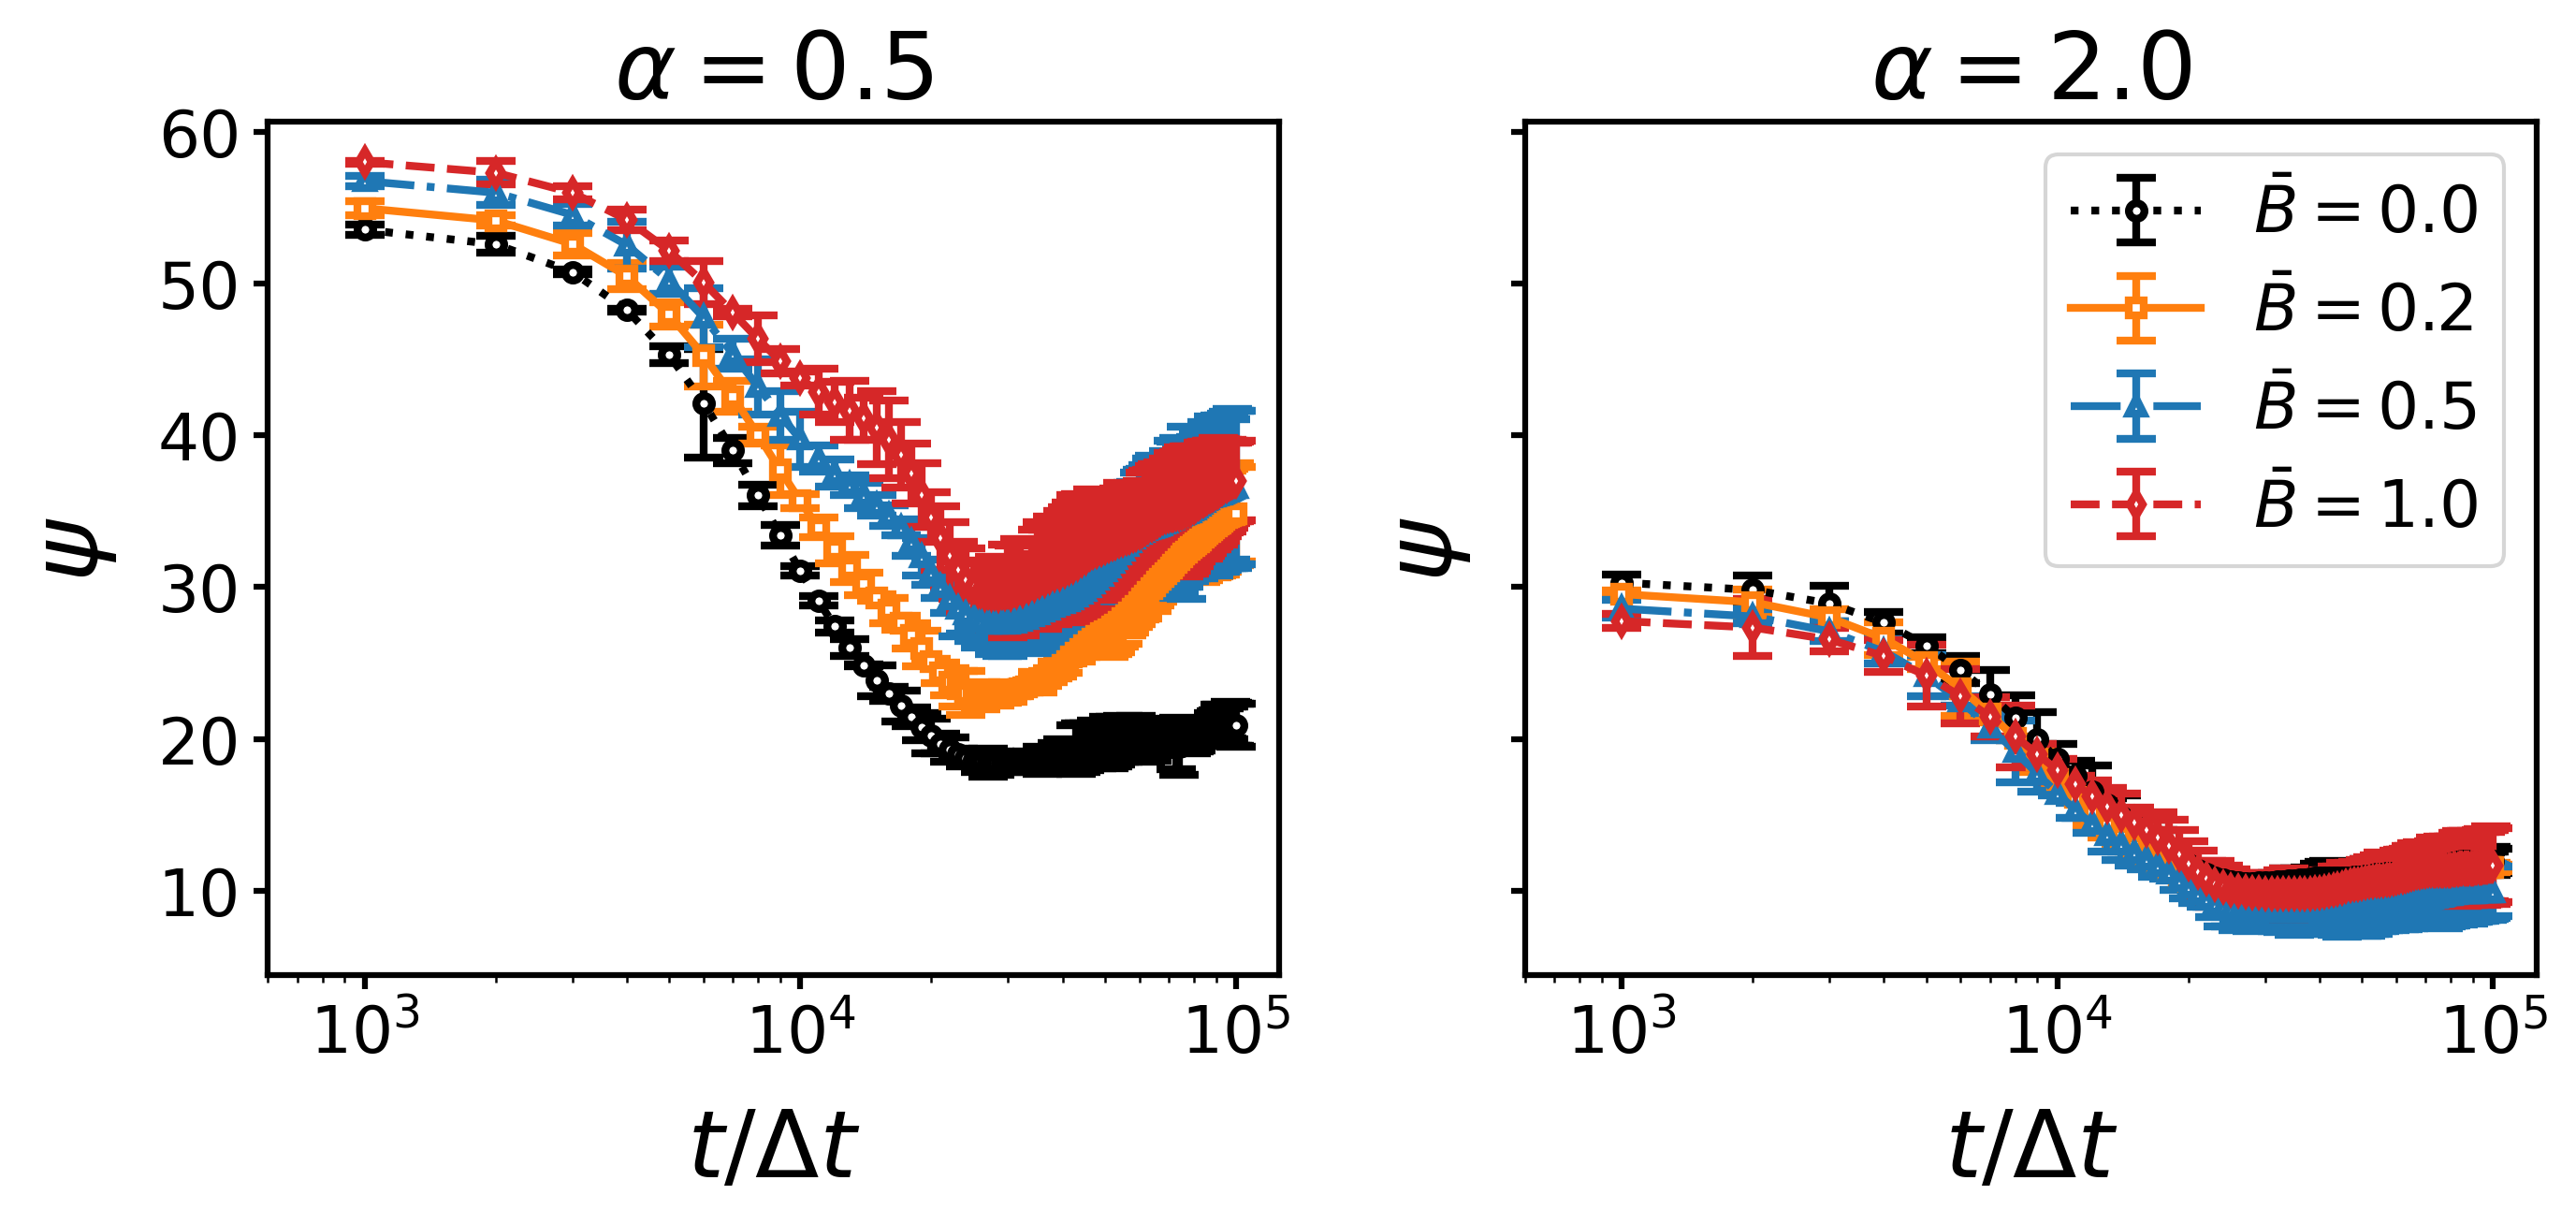
\includegraphics[scale = 0.4]{figures/results/paper1/psi-vs-t.png}
    \caption{Time-dependence of the average angle $\psi$ between the particle axis and the 
            interface normal for oblate ($\alpha=0.5$) and prolate ($\alpha=2$) particles at different 
            magnetic field strength $\bar{B}$. Errorbars indicate the standard deviation taken over three 
            independent simulation runs. The angle between between the particles and the interface normal generally 
            approaches the energetically preferred value ($0^\circ$ for oblate particls, $90^\circ$ for prolate particles).
            The average angle changes most rapidly around $10^4$ timesteps.}
    \label{fig:psi_time}
\end{figure}


Hence the prolate particles remain mostly aligned with the interface
even in the stronger applied magnetic fields. We plot the interface angle of bijels
stabilized by ellipsoidal particles at the final timestep to demonstrate the differences
that the application of magnetic fields have on the particle monolayer.

\begin{figure}
    \centering
    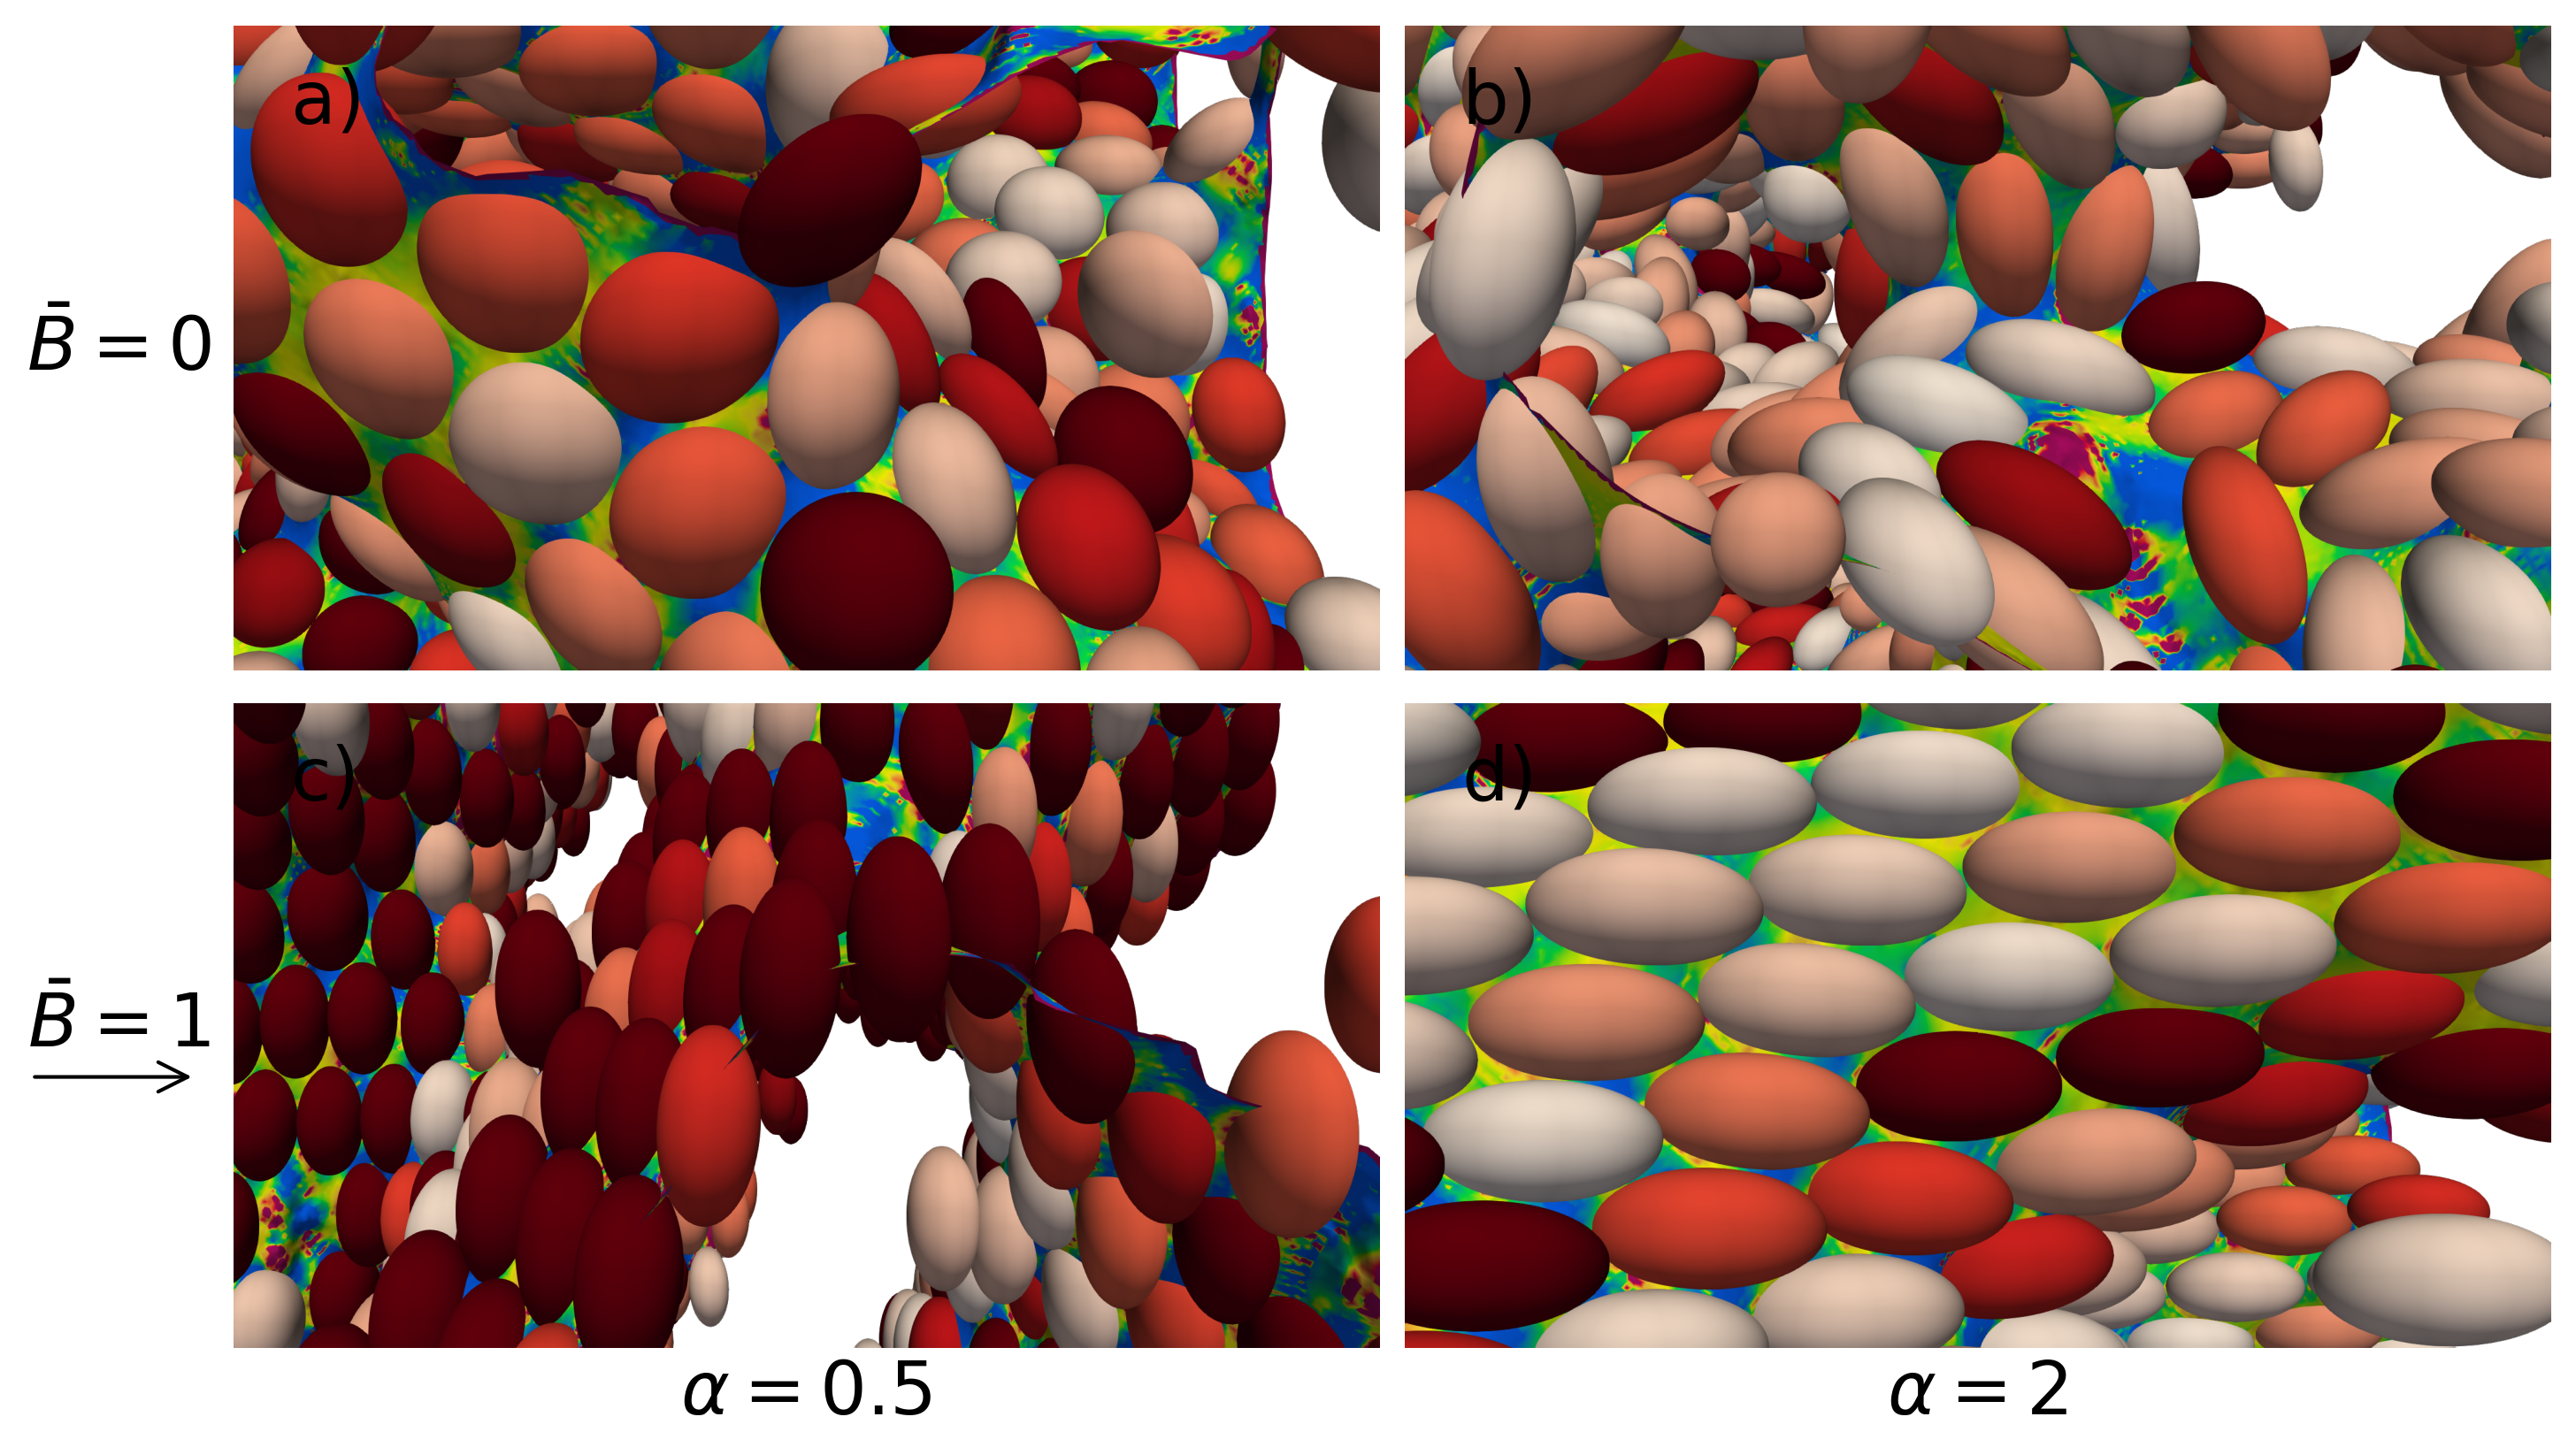
\includegraphics[scale = 0.4]{figures/results/paper1/psi_concat.png}
    \caption{Visualizations of the particle monolayer at the last timestep shaded with the interface angle of each particle in red. The top and bottom
             rows correspond to snapshots of bijels with no field and a field strength of $\bar{B} = 1$ applied. We see that the oblate particles flip
             out of the interface into a non energetically favored position while the bijels stabilized with prolate particles tilt out of the interface
             but are less likely to flip out.}
    \label{fig:psi_viz_ss}
\end{figure}

Hence the prolate particles remain mostly aligned with the interface
even in the stronger applied magnetic fields. We plot the interface angle of bijels
stabilized by ellipsoidal particles at the final timestep to demonstrate the differences
that the application of magnetic fields have on the particle monolayer.

\begin{figure}
        \centering
        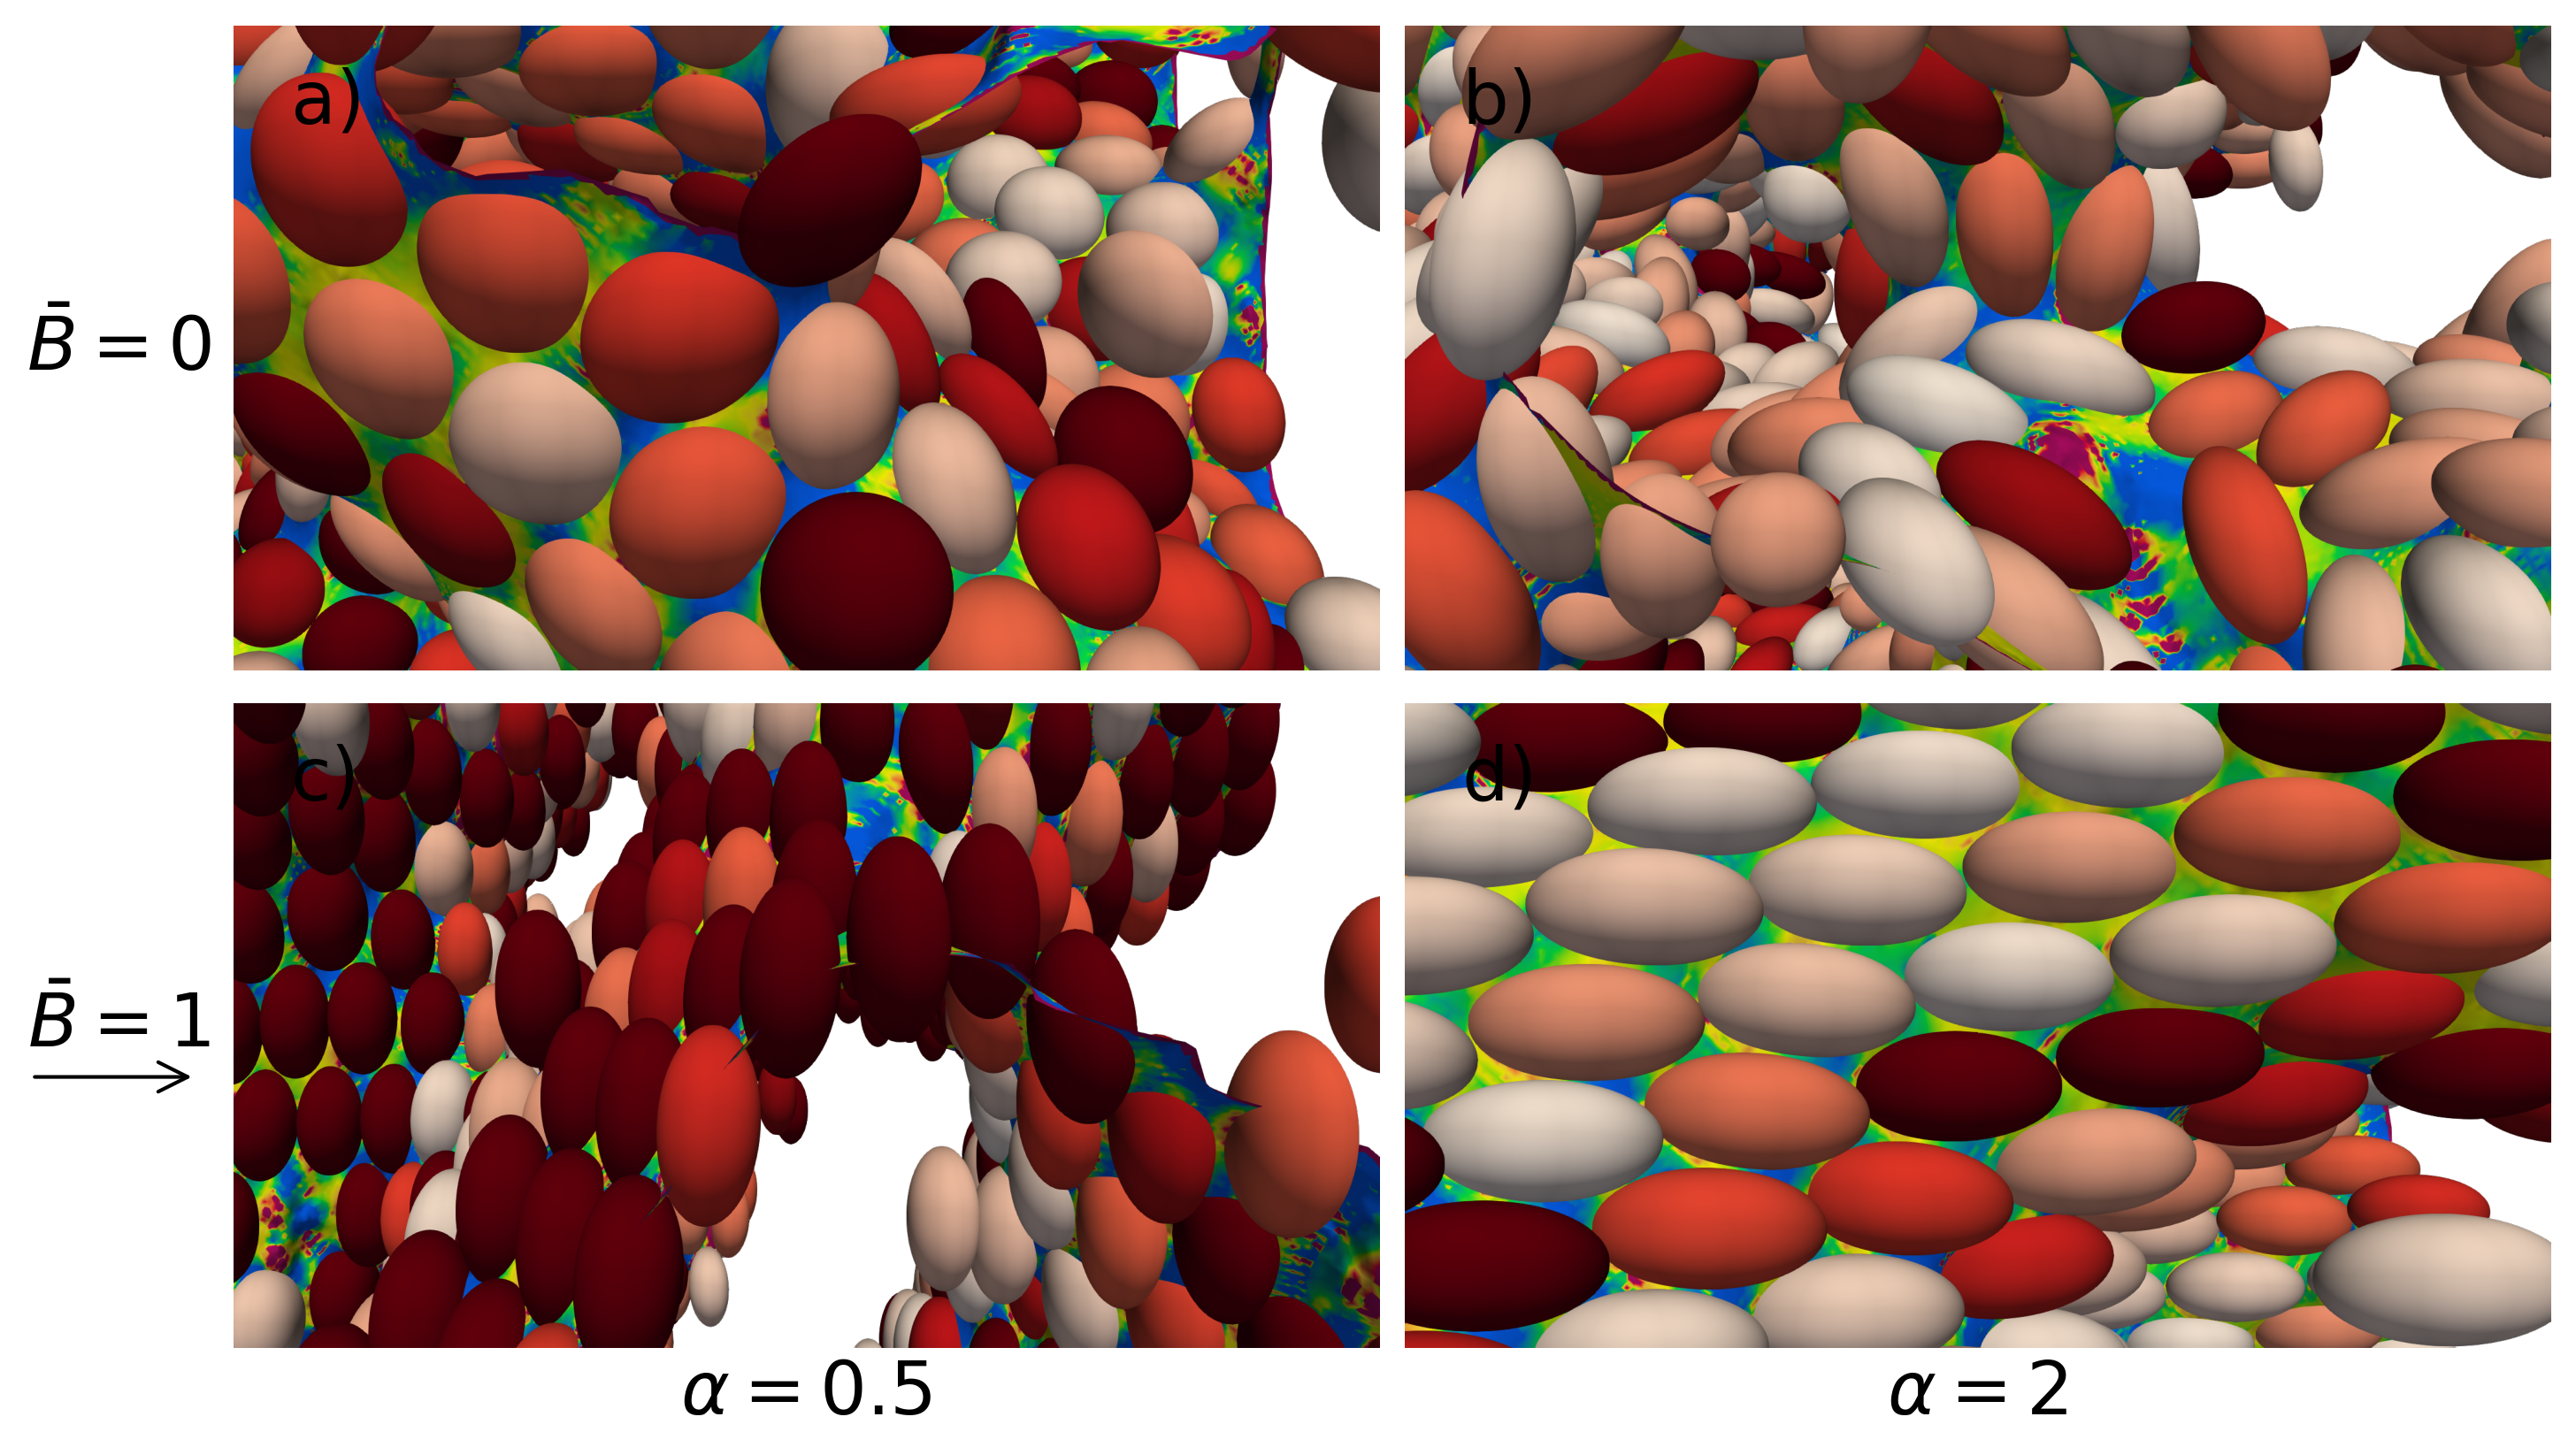
\includegraphics[scale = 0.4]{figures/results/paper1/psi_concat.png}
        \caption{Visualizations of the particle monolayer at the last timestep shaded with the interface angle of each particle in red. The top and bottom
                 rows correspond to snapshots of bijels with no field and a field strength of $\bar{B} = 1$ applied. We see that the oblate particles flip
                 out of the interface into a non energetically favored position while the bijels stabilized with prolate particles tilt out of the interface
                 but are less likely to flip out.}
        \label{fig:psi_viz_ss}
\end{figure}

From Figure \ref{fig:psi_viz_ss} We can see the differences in the particle alignment to the interface characerizing the differences in $\psi$ observed. Oblate
particles can be seen to tilt out of the interface more readily than prolate particles at the same magnetic field strength. Due to the strong surface tension
between the fluids, the particles are strongly adsorbed onto the interface. We also see that the arrangement of particles on the interface is modified through the
application of the magnetic field for both particle morphologies. We can obtain quantitative metrics regarding this ordering using the Steinhardt 2 and 6 fold
order parameters, $\langle Q2 \rangle$ and $\langle Q6 \rangle$. 

This parameter has been used extensively to characterize nucleation rates, glass transitions of colloidal systems and crystal structure transitions of ceramics 
and colloidal crystals. \cite{vagberg_glassiness_2011, besseling_three-dimensional_2007, schall_structural_2007} The original implementation has been further 
improved through the use an averaged bond order parameter, adding the next nearest neighbor to the neighbor list or utilizing voronoi cells to define the 
neighbor list instead of a cutoff distance. The latter provides a more robust definition of the neighbor list, without needing to assume the structure of 
the particles and is implemented in the package Freud. \cite{ramasubramani_freud_2020} This method has been used to characterize the jamming of discs at 
interfaces. \cite{ozawa_jamming_2012}

We select $\langle Q6 \rangle$ and $\langle Q2 \rangle$ as the bond order parameters to calculate as We am interested in identifying the point when ordering 
of the material changes. Kapfer et al. demonstrated that only using $\langle Q6 \rangle$ to identify the ordering of particles in the system can result in 
false positives when the particles have icosahedral or amorphous structure. \cite{kapfer_jammed_2012} Mickel et al. showed how increasing deviations from 
$\langle Q2 \rangle = 0$ can be used to characterize increasing disorder in a system. \cite{mickel_shortcomings_2013} By plotting $\langle Q6 \rangle$ and 
$\langle Q2 \rangle$, we will be able to identify changes in the local ordering of the system even if We cannot directly assess the local structure quantitatively.

\begin{figure} 
    \centering 
    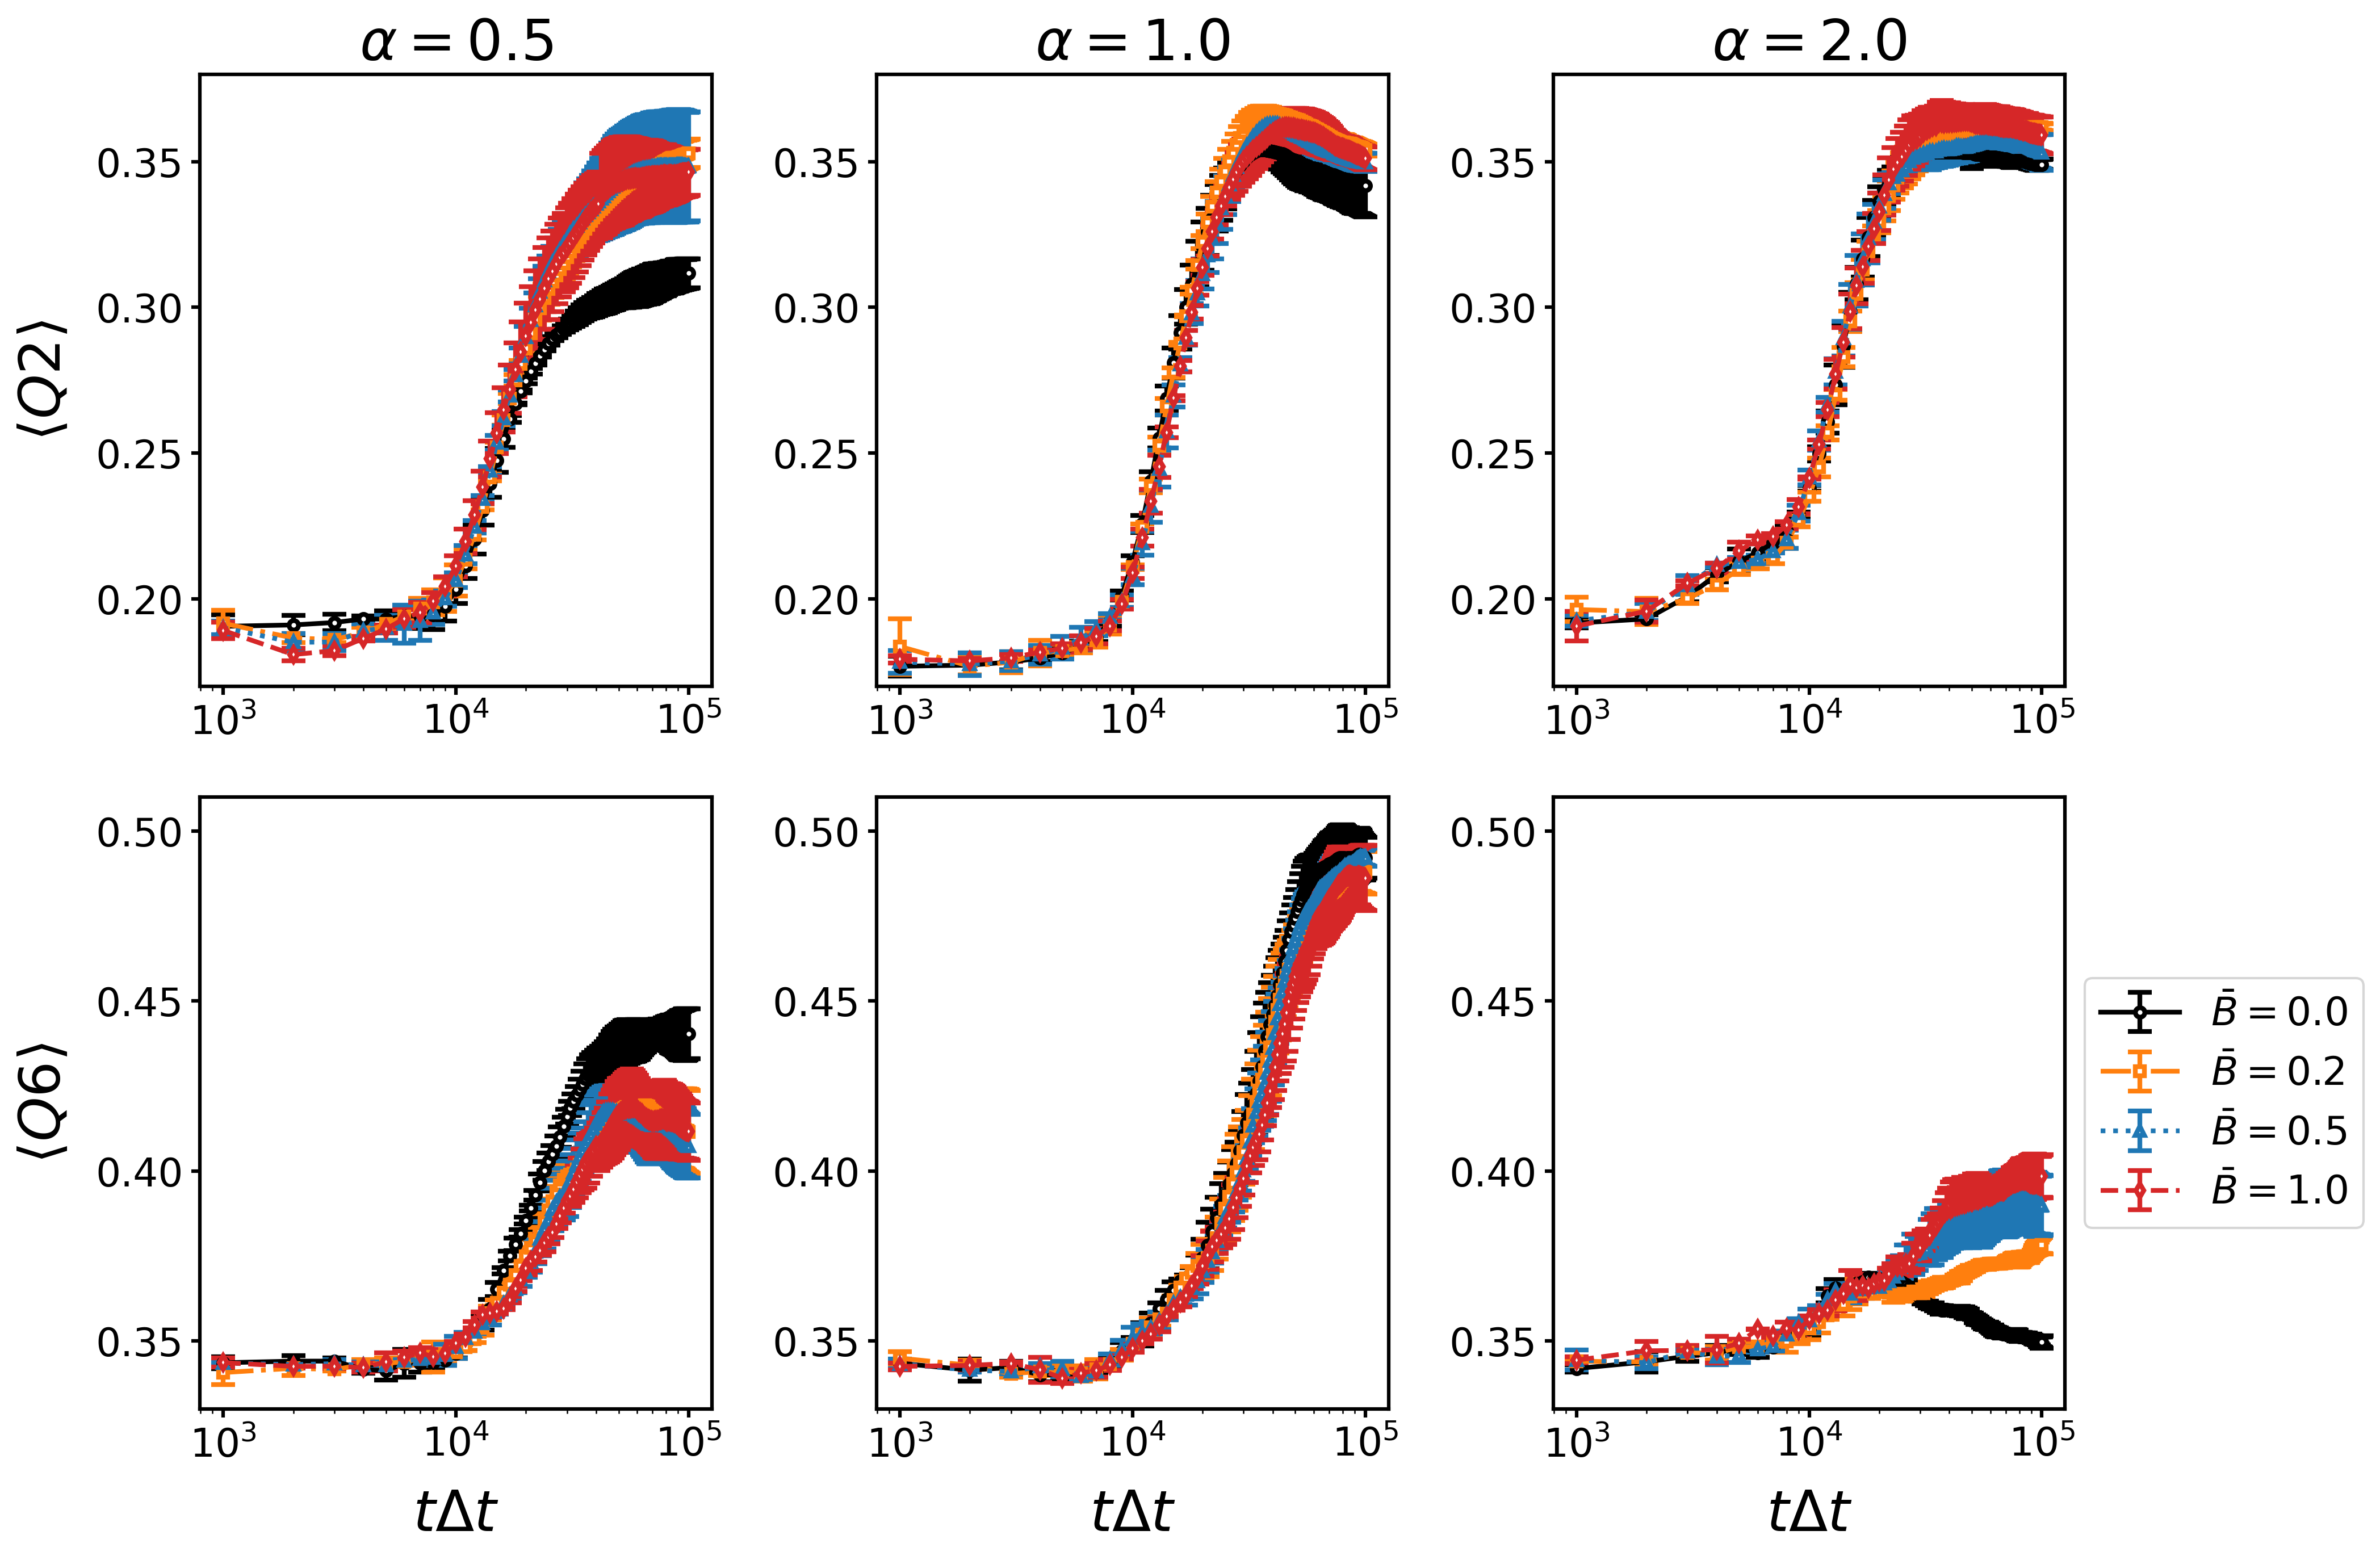
\includegraphics[width=\columnwidth]{figures/results/paper1/steinhardt_vs_coverage.png} 
    \caption{Time dependence of the mean two and six fold symmetry parameter, $\langle Q2 \rangle$ and $\langle Q6 \rangle$ 
    for bijels stabilized with oblate(left), spherical(middle) and prolate(right) particles. We use $\langle Q2 \rangle$ as an
    indicator of global particle translational order while $\langle Q6 \rangle$ is an indicator of local order.} 
    \label{fig:steinhardt_coverage} 
\end{figure}

From Figure \ref{fig:steinhardt_coverage}, we see an increase in disorder in all the bijel systems characterized as an increase in $\langle Q2 \rangle$. 
This is a characteristic of how the particles were initialized and move once the simulation is initiated. The particles are initialized to be randomly placed 
in the simulation domain with roughly equal spacing. As the interface sweeps through the simulation domain, particles irreversibly adsorb onto the interface 
and move with the interface until the bijel jams. We see that $\langle Q2 \rangle$ is magnetic field dependent for oblate particles but not for the spherical 
and prolate particles. We also see an aspect ratio dependence on the values characterized as differences in the time evolution of $\langle Q2 \rangle$. This 
arises due to the differences in the aspect ratio of the particle causing them to arrange differently on the interface as the bijel microstructure evolves.

An increase in $\langle Q6 \rangle$ can indicate an increase in the number of particles adopting icosahedral symmetry at the interface of the amorphous 
interface. \cite{kapfer_jammed_2012} However due to the amorphous nature of the arrangement of particles at the particle monolayer, we use this parameter 
only to gauge changes in local arrangements of particles at the interface and make no commentary on specific interfacial arrangements. For oblate particles, 
we characterize a reduction in local order as the applied field strength is increased, consistent with the increase in $\langle Q2 \rangle$. For prolate 
particles, we observe that $\langle Q6 \rangle$ increases with the applied field. This indicates that the application of the field causes particles to have 
increased local order, even if we see no discernible changes in $\langle Q2 \rangle$. 

The application of the magnetic field affects the prolate and oblate particle differently due to their aspect ratio. At interfaces, rod-like particles 
prefer to orient themselves in an end to end fashion. \cite{eatson_capillary_2023} Disc-like particles have been shown to prefer stacking. \cite{dabat_mesoscale_2018} 
Application of the magnetic field and the presence of an interface will constrain the rotation of the particles, meaning that naturally rods will pack better at 
interfaces than discs as the magnetic field causes the particles to align to the field. This better packing at the interface manifests as greater local ordering 
Next, we analyze how these local toplogical changes affect the microstructure of the bijel by analyzing the channel size distribution of the bijels.

As hypothesized above, the alignment of the particle dipole axis with
the magnetic field reduces the steric constraints within the interface.
To corroborate this idea, we analyzed the radial distribution function
(RDF) of the particles, the calculation of which is detailed in Section
\ref{section:radial_distribution} The time-evolution of the RDFs for the three particle shapes and
varying magnetic flux density is illustrated in Figure \ref{fig:rdf}.

\begin{figure}
\centering
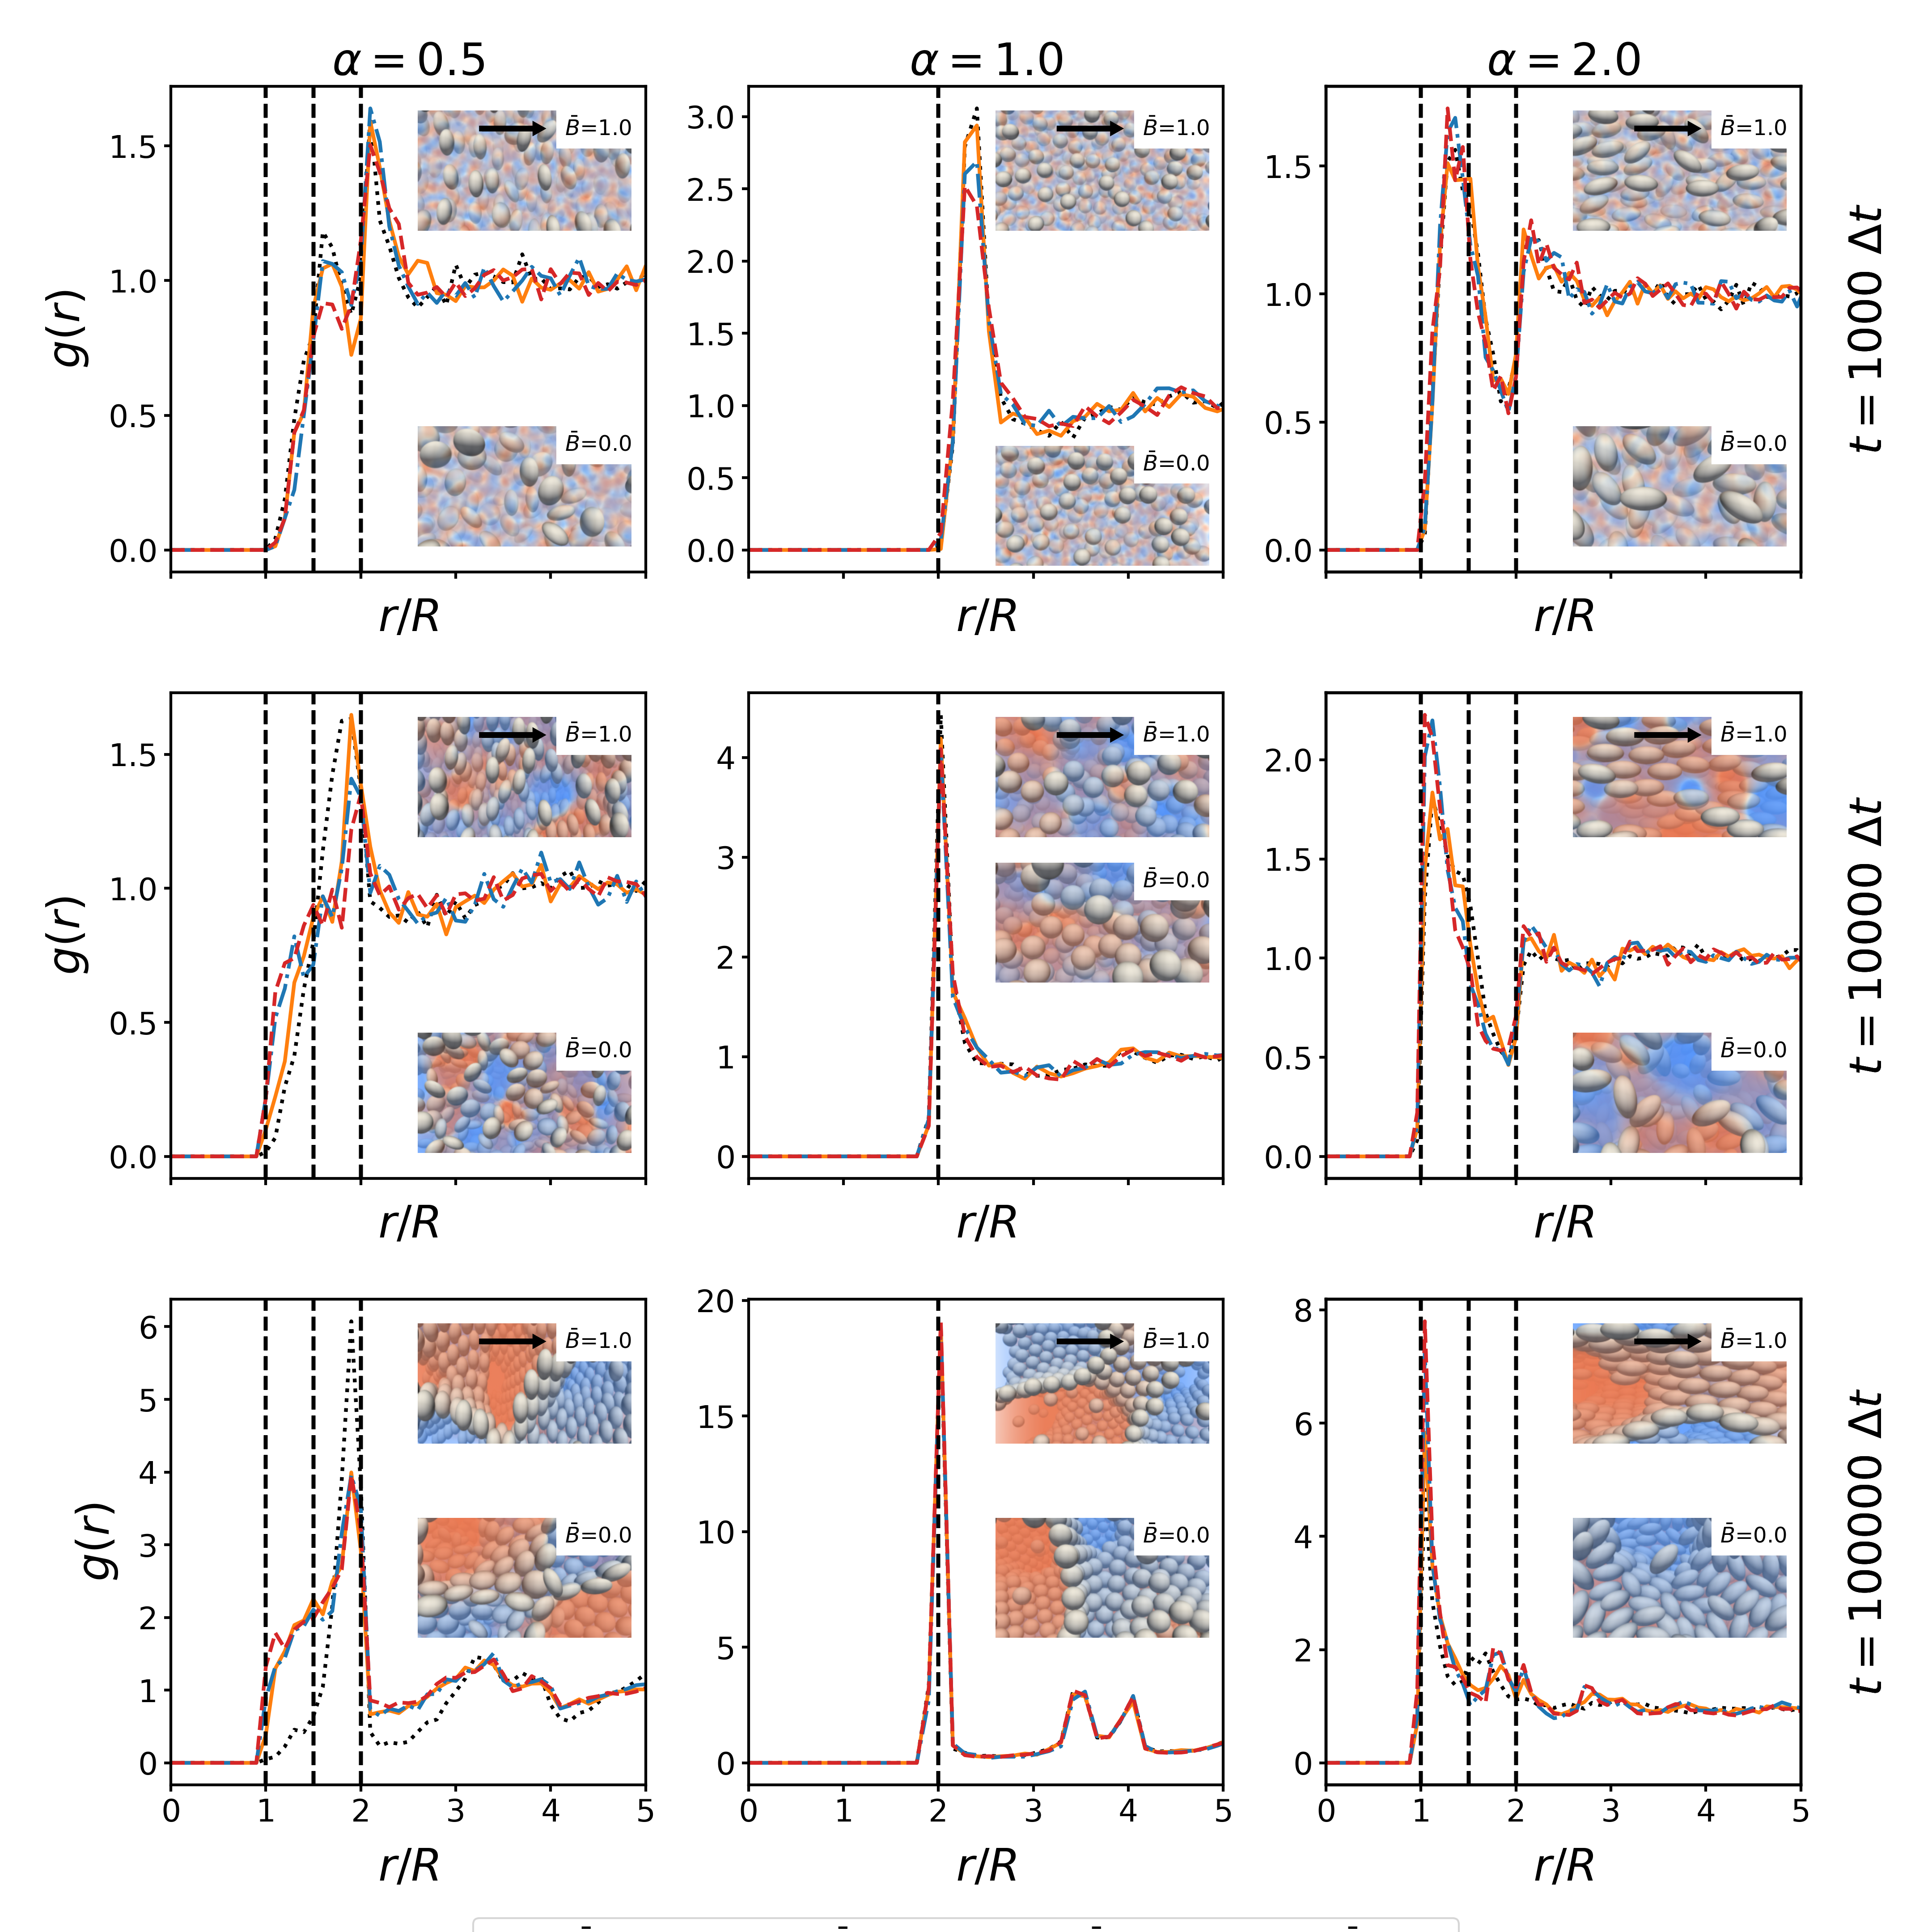
\includegraphics[width=\textwidth]{figures/results/paper1/rdf_compare_time.png}
\caption{Time-evolution of the radial distribution function $g(r)$ of the particles at different magnetic 
        field strength $\bar{B}$. The radial distribution function is shown at $10^3$, $10^4$, and $10^5$ timesteps. 
        The distance $r$ is normalized by the radius $R=\max(R_\parallel,R_\perp)$ of the larger particle axis. The peaks 
        illustrate the packing of particles in the interface. Dashed lines indicate the side-by-side, tip-to-tip, 
        and side-to-tip configuration of particle pairs. For spherical particles, the three values are identical. 
        The insets show snapshots of the particle arrangement with and without magnetic field at the respective timesteps. 
        The direction of the magnetic field is indicated by arrows.}
\label{fig:rdf}
\end{figure}
